\documentclass[11pt]{article}

\usepackage[a4paper,margin=1in]{geometry}
\usepackage{amsmath,amssymb,amsfonts}
\usepackage{bm}
\usepackage{graphicx}
\usepackage{booktabs}
\usepackage{array}
\usepackage{float}
\usepackage{caption}
\usepackage[hidelinks]{hyperref}
\usepackage[numbers,sort&compress]{natbib}

\graphicspath{{figures/}}

\title{Non-Markovian Gravitational Collapse: Structural Memory, Wave Emission, and Recoverability Loss}
\author{Stephen Atalebe}
\date{}

\begin{document}
\maketitle

\begin{abstract}
Gravitational collapse is commonly parameterized by instantaneous or near-instantaneous source variables, including mass, compactness, pressure support, rotation, anisotropy, curvature, and equation-of-state structure. This paper develops a complementary source-side formulation in which collapse is treated as an effectively non-Markovian process. The central claim is not that general relativity is modified at the level of gravitational-wave propagation. The claim is narrower: an effective source state can be incomplete if it omits retained compression history. A collapse-state vector is introduced in terms of structural reserve, recoverability, coherence, and memory. The memory component is defined through a causal kernel over prior collapse-history observables, such as compression rate, shear, anisotropic stress, entropy production, accretion variability, curvature strain, or quadrupole deformation. The framework predicts that two systems matched in their instantaneous state can generate different subsequent waveform residuals if their prior histories differ and if the memory coordinate remains dynamically coupled to collapse evolution. The memory term is framed as an effective source correction: when unresolved short-timescale microphysics, turbulent cascades, anisotropic transport, or radiation-hydrodynamic structure are reduced to macroscopic variables, the remaining equations need not be memory-free.

The paper contains two phases. The first phase gives an executable scalar validation. A matched-state toy model is constructed in which smooth and bursty collapse histories are reset to identical values of \(R\), \(\dot R\), and \(A\) at a reference time \(t_\ast\), while retaining different memory values. In the amplified fixed-history scan, the retained memory contrast is \(\Delta M_{\rm coll}(t_\ast)=4.839\times10^{-3}\). The Markovian null gives a post-match waveform residual norm of \(2.10\times10^{-10}\), whereas the memory-coupled case with \(\lambda_{\rm mem}=0.20\) gives \(9.44\times10^{-4}\). Synthetic colored-noise injections, a three-detector network test, and a network signal-to-noise scan further show that the memory-on residual is strongly separable from the Markovian null under the adopted toy detector model. The second phase gives a disciplined implementation architecture for lifting the scalar variables into field-valued \(3+1\) general-relativistic hydrodynamic variables. No full numerical-relativity implementation is claimed. The resulting contribution is a falsifiable theory and validation architecture for source-side structural memory in gravitational collapse.
\end{abstract}

\section{Introduction}

The direct detection of gravitational waves from binary black-hole coalescence opened an observational regime in which strong-field gravity and compact-object dynamics can be studied through waveform structure \citep{Abbott2016GW150914}. Since then, gravitational-wave astronomy has moved from event confirmation to source diagnosis. Waveforms are now used to infer masses, spins, tidal structure, merger dynamics, propagation effects, and possible departures from general relativity. In parallel, gravitational waves have become probes of cosmology through standard sirens, modified gravitational-wave propagation, and tests of late-time cosmic acceleration \citep{Belgacem2018ModifiedGW,Belgacem2019TestingMG,Tagliazucchi2025StandardSiren}.

A related development has occurred in gravitational-collapse modelling. Core-collapse supernovae, compact-object mergers, nonspherical collapse, primordial collapse, and nonsingular collapse models increasingly treat gravitational-wave emission as a probe of hidden source dynamics. Recent work on core-collapse supernovae emphasizes that gravitational waves may encode information about progenitor structure, proto-neutron-star contraction, hydrodynamic instabilities, turbulent motion, nuclear equation-of-state effects, and rotation \citep{Muller2017CCSN,Muller2026CCSNReview,Murphy2026Progenitor}. Simulations of nearly equal-mass progenitors with different internal structures can produce different waveform features in amplitude, energy release, and time-frequency evolution, indicating that gravitational waves can retain information about the interior path to collapse \citep{Murphy2026Progenitor}. This makes gravitational-wave astronomy a natural setting in which to ask whether collapse is fully described by instantaneous source variables, or whether retained source history should be written explicitly.

A separate but conceptually adjacent development concerns gravitational-wave memory. Gravitational-wave memory is a non-oscillatory radiative contribution to the strain that can leave a permanent displacement after the wave has passed \citep{Favata2010Memory,Lasky2016Memory}. Recent studies have examined detectability prospects for memory with current and future observatories, including Bayesian approaches for LISA and extensions beyond general relativity \citep{Cogez2026LISAMemory,Gasparotto2026BeyondGRMemory}. The memory used in this paper is different. Source-side structural memory is an internal dynamical-history coordinate of the source before or during emission. Gravitational-wave memory is a radiative spacetime effect. The proposed bridge is conditional: retained source history may alter the matter and geometry that generate the waveform, and therefore may modulate burst morphology, low-frequency residuals, ringdown structure, or memory-like waveform components.

The working hypothesis is simple. Collapse systems that are equivalent under a selected instantaneous state can produce distinguishable gravitational-wave signatures when their prior compression histories differ. This claim is deliberately conservative. It does not require modifying gravitational-wave propagation. It asks whether the effective source dynamics feeding the waveform are complete when prior structural history is excluded.

The paper proceeds in two phases. The first phase formulates and tests the scalar theory. It defines a causal source-memory coordinate, embeds it in a collapse-state vector, constructs a matched-state toy model, and tests memory-on versus memory-off distinguishability in synthetic colored noise and in a three-detector network architecture. The second phase gives a \(3+1\) general-relativistic hydrodynamic uplift. It shows how the scalar variables can be interpreted as projections of field-valued quantities and how a memory tensor could enter conservative GRHD source terms. The second phase is an implementation architecture, not a claim of a completed numerical-relativity simulation.

\section{Effective Source Memory in Collapse}
\label{sec:source_memory}

A Markovian effective source model assumes that the future evolution of a collapsing system is conditionally determined by its present state. If \(\bm{x}(t)\) denotes the chosen source variables, then
\begin{equation}
\frac{d\bm{x}}{dt}=\bm{F}\left(\bm{x}(t),t;\bm{\theta}\right),
\end{equation}
where \(\bm{\theta}\) denotes fixed parameters or slowly varying nuisance quantities. Under this description, prior history matters only through its influence on the current value of \(\bm{x}(t)\). Once the present state is fixed, the path taken to reach that state has no independent dynamical role.

This assumption is useful, but it is not always physically neutral. Realistic collapse systems can carry prior structural information through anisotropy, turbulent cascades, shell interactions, angular-momentum redistribution, accretion history, entropy production, neutrino transport, magnetic stresses, phase transitions, and curvature strain. A slowly compressed object and a violently perturbed object need not be dynamically equivalent merely because a selected instantaneous diagnostic agrees. The issue is not whether the field equations of general relativity are valid. The issue is whether the effective source state is complete.

The memory term can be viewed as an effective-field or reduced-order correction rather than as an arbitrary addition. When unresolved microphysics or short-timescale transport is integrated out, the reduced macroscopic system can inherit relaxation, hysteresis, or finite-memory terms. In this sense, the proposed source-memory coordinate records part of the information flow from ordered macroscopic collapse into smaller-scale turbulent, anisotropic, or dissipative degrees of freedom. A memory-free model discards this pathway once the instantaneous state is specified; the present framework asks whether any part of that retained path remains predictive of the later waveform.

Source-side structural memory is defined here as retained information about the prior collapse path that influences later source dynamics or emitted radiation. It is written as a causal memory functional,
\begin{equation}
M_{\rm coll}(t)=\int_{t_0}^{t}K(t,t')\,\Xi(t')\,dt',
\label{eq:memory_kernel}
\end{equation}
where \(K(t,t')\) is a causal memory kernel and \(\Xi(t')\) is a collapse-history observable. The kernel determines how strongly past states influence the present. A short-range kernel approaches the Markovian limit. A long-range kernel allows distant prior states to retain dynamical influence. In a core-collapse supernova context, \(\Xi\) may represent turbulent stress, proto-neutron-star contraction rate, accretion variability, entropy production, neutrino-driven anisotropy, or quadrupole deformation. In compact-object collapse, it may represent curvature strain, tidal deformation, angular-momentum redistribution, or near-horizon anisotropy.

The scalar collapse-state vector is
\begin{equation}
\hat{\phi}_{\rm coll}(t)=\left(H_{\rm coll}(t),R_{\rm coll}(t),S_{\rm coll}(t),M_{\rm coll}(t)\right).
\label{eq:collapse_vector}
\end{equation}
Here \(H_{\rm coll}\) represents structural reserve against runaway collapse, \(R_{\rm coll}\) represents recoverability, \(S_{\rm coll}\) represents coherence of the collapsing configuration, and \(M_{\rm coll}\) represents retained collapse history. The formulation is intentionally effective. It is not a replacement for numerical relativity, hydrodynamic simulation, or general-relativistic perturbation theory. It is a state-space completion of the source description.

\begin{table}[t]
\centering
\caption{Illustrative physical proxies for the collapse-state variables. The entries are not unique definitions; they indicate possible instantiations for simulation-level tests.}
\begin{tabular}{lll}
\toprule
Component & State-space role & Possible collapse proxies \\
\midrule
\(H_{\rm coll}\) & Structural reserve & pressure support, angular momentum, magnetic support, thermal reserve \\
\(R_{\rm coll}\) & Recoverability & shock revival tendency, bounce capacity, remnant stability, horizon-avoidance margin \\
\(S_{\rm coll}\) & Coherence & mode organization, turbulence level, anisotropy, shell-crossing disorder \\
\(M_{\rm coll}\) & Retained history & integrated shear, entropy production, accretion variability, curvature strain \\
\bottomrule
\end{tabular}
\label{tab:collapse_proxies}
\end{table}

The recoverability component requires careful framing. Within the effective state-space description, terminal or singular collapse corresponds to the limit in which recoverable state-space structure is lost, \(R_{\rm coll}\to0\). This is a diagnostic statement, not a replacement for geometric singularity definitions. It indicates that the model treats singular or terminal behaviour as a loss of recoverable source structure, while leaving the geometric problem of singularity formation to relativistic theory.

\section{Scalar Projection and Tensor-Valued Generalization}
\label{sec:tensor_generalization}

The collapse-state vector is written in scalar form for clarity. It should not be read as a claim that gravitational collapse is intrinsically described by four scalar observables. In a realistic three-dimensional relativistic hydrodynamic or magnetohydrodynamic setting, each component may be field-valued, tensor-valued, or represented by a reduced-order projection of a higher-dimensional structure.

The scalar vector in Eq.~\eqref{eq:collapse_vector} is therefore interpreted as a projection of a field-valued state,
\begin{equation}
\hat{\Phi}_{\rm coll}(t,\mathbf{x})=\left(\mathcal{H}(t,\mathbf{x}),\mathcal{R}(t,\mathbf{x}),\mathcal{S}(t,\mathbf{x}),\mathcal{M}(t,\mathbf{x})\right),
\end{equation}
through operators
\begin{equation}
H_{\rm coll}=\Pi_H[\mathcal{H}],\quad R_{\rm coll}=\Pi_R[\mathcal{R}],\quad S_{\rm coll}=\Pi_S[\mathcal{S}],\quad M_{\rm coll}=\Pi_M[\mathcal{M}].
\end{equation}
The projection operators may represent volume averages, mass-weighted averages, mode amplitudes, principal components, spherical-harmonic coefficients, quadrupole-weighted summaries, or reduced-order embeddings. This generalization allows the same conceptual state-space structure to be used across toy models, numerical-relativity simulations, core-collapse supernova catalogues, and observational waveform inference without requiring the physical system itself to be scalar.

\section{Source Memory and Wave Emission}
\label{sec:wave_coupling}

Gravitational waves are generated by time-dependent mass-energy dynamics. In the weak-field quadrupole approximation, the strain is related to the second time derivative of the mass quadrupole moment,
\begin{equation}
h_{ij}^{\rm TT}(t)\propto \frac{2G}{c^4D}\frac{d^2 Q_{ij}^{\rm TT}}{dt^2},
\end{equation}
where \(D\) is the distance to the source and \(Q_{ij}^{\rm TT}\) is the transverse-traceless quadrupole moment. In strong-field systems, full relativistic treatments are required, but the source-side point remains: waveform structure depends on the dynamical trajectory of the emitting system.

A memory-completed effective waveform can be written schematically as
\begin{equation}
h(t)=h_{\rm inst}(t;\bm{\theta}_{\rm inst})+\epsilon\,h_{\rm srcM}\left[t;H_{\rm coll},R_{\rm coll},S_{\rm coll},M_{\rm coll}\right],
\label{eq:waveform_memory}
\end{equation}
where \(h_{\rm inst}\) is the waveform predicted from instantaneous source variables and \(h_{\rm srcM}\) is the source-memory contribution. Equation~\eqref{eq:waveform_memory} is an effective decomposition, not a claim that gravitational-wave propagation is modified.

A direct test follows. Consider two source trajectories \(A\) and \(B\) satisfying
\begin{equation}
\bm{x}_A(t_\ast)=\bm{x}_B(t_\ast),
\qquad
M_{{\rm coll},A}(t_\ast)\neq M_{{\rm coll},B}(t_\ast).
\end{equation}
A purely Markovian effective source model predicts equivalent future evolution up to noise and unresolved nuisance parameters. A non-Markovian source model predicts residual differences,
\begin{equation}
\Delta h(t>t_\ast)=h_A(t)-h_B(t)\neq0,
\end{equation}
with residual structure correlated with the difference in \(M_{\rm coll}\).

A central risk is degeneracy. A waveform residual attributed to source-side memory may instead reflect an incomplete instantaneous model. Missing equation-of-state dependence, unresolved magnetic-field topology, rotation-profile uncertainty, neutrino-transport approximations, progenitor composition, detector noise, or numerical error can all produce residual structure. The distinction proposed here is operational. A missing-physics residual is reducible to an enlarged instantaneous state. A genuine source-memory residual is not. Let the instantaneous state be expanded to
\begin{equation}
\bm{x}_{\rm ext}(t)=\left[\bm{x}(t),\bm{q}_{\rm EOS}(t),\bm{q}_{B}(t),\bm{q}_{\Omega}(t),\bm{q}_{\nu}(t),\bm{q}_{\rm num}(t)\right].
\end{equation}
A memory interpretation is justified only if waveform residuals remain correlated with prior-history observables after conditioning on \(\bm{x}_{\rm ext}(t_\ast)\). Symbolically,
\begin{equation}
\Delta h(t>t_\ast)\not\!\perp\!\!\!\perp M_{\rm coll}(t_\ast)\,\big|\,\bm{x}_{\rm ext}(t_\ast).
\end{equation}
If this conditional dependence vanishes, the memory term is not required. If it persists across controlled simulations, waveform families, and nuisance-parameter expansions, the source dynamics are effectively non-Markovian.

\section{Toy-Model Methods}
\label{sec:toy_methods}

The toy model is designed to isolate the central claim under controlled conditions. It does not attempt to reproduce realistic relativistic collapse. Let \(R(t)\) denote a dimensionless collapse coordinate, normalized so that larger \(R\) corresponds to a more extended configuration and smaller \(R\) corresponds to stronger compression. The memory-free model is
\begin{equation}
\ddot{R}+\gamma\dot{R}+\omega^2R=-\frac{\mu}{(R+\epsilon_R)^2}+F_{\rm drive}(t),
\label{eq:toy_markovian}
\end{equation}
where \(\gamma\) is an effective damping coefficient, \(\omega\) is a stiffness scale, \(\mu\) controls inward forcing, \(\epsilon_R\) regularizes the small-radius limit, and \(F_{\rm drive}\) is an imposed compression history. The implemented version also includes a soft-core regularizer to prevent the diagnostic coordinate from crossing \(R=0\). The memory-completed model is
\begin{equation}
\ddot{R}+\gamma\dot{R}+\omega^2R=-\frac{\mu}{(R+\epsilon_R)^2}+F_{\rm drive}(t)+\lambda_{\rm mem}M_{\rm coll}(t),
\label{eq:toy_nonmarkovian}
\end{equation}
where \(\lambda_{\rm mem}\) controls coupling between retained source history and present collapse acceleration.

With an exponential kernel, the memory integral is evolved as
\begin{equation}
\dot{M}_{\rm coll}=\frac{1}{\tau_M}\left[\Xi(t)-M_{\rm coll}(t)\right],
\label{eq:toy_memory_ode}
\end{equation}
where
\begin{equation}
\Xi(t)=\dot{R}^2(t)+\beta A^2(t).
\label{eq:toy_history_observable}
\end{equation}
Here \(A(t)\) is a dimensionless anisotropy or shear proxy. In the toy model, the smooth history and bursty history use different pre-matching drives. At \(t_\ast\), \(R\), \(\dot R\), and \(A\) are explicitly reset to the same values, while \(M_{\rm coll}\) is not reset. After \(t_\ast\), both trajectories evolve under identical forcing.

The waveform proxy is constructed from
\begin{equation}
Q_{\rm toy}(t)=R^2(t)\left[1+\eta A(t)\right],
\end{equation}
and
\begin{equation}
h_{\rm toy}(t)=C_h\frac{d^2Q_{\rm toy}}{dt^2}.
\label{eq:toy_waveform}
\end{equation}
The memory-associated residual is
\begin{equation}
\Delta h_M(t)=h_{{\rm toy},A}(t)-h_{{\rm toy},B}(t),\qquad t>t_\ast.
\end{equation}
The comparison is performed using a fixed-history scan: the pre-matching histories are generated once, the retained \(\Delta M_{\rm coll}(t_\ast)\) is held fixed, and only the post-matching coupling \(\lambda_{\rm mem}\) is scanned. This prevents the memory contrast itself from changing across the coupling grid.

The test can fail. It is rejected if the trajectories cannot be matched at \(t_\ast\), if \(M_{{\rm coll},A}(t_\ast)\) and \(M_{{\rm coll},B}(t_\ast)\) do not differ, if the waveform residual for \(\lambda_{\rm mem}>0\) is not larger or more structured than the Markovian residual, or if the apparent residual can be eliminated by adding ordinary instantaneous variables to the matched state.

\section{Toy-Model Results}
\label{sec:toy_results}

The amplified-history fixed scan provides the primary toy-model demonstration. The two histories were forced at \(t_\ast\) to share identical \(R\), \(\dot R\), and \(A\), giving \(\delta_{\rm match}=0\). The retained memory coordinate was preserved, producing
\begin{equation}
\Delta M_{\rm coll}(t_\ast)=4.839\times10^{-3}.
\end{equation}
In the Markovian null case, \(\lambda_{\rm mem}=0\), the post-match waveform residual norm was \(2.10\times10^{-10}\). When the same fixed memory contrast was evolved with nonzero memory coupling, the residual increased monotonically, reaching \(9.44\times10^{-4}\) at \(\lambda_{\rm mem}=0.20\). The largest-coupling residual is approximately \(4.49\times10^6\) times the Markovian null. Thus, after exact instantaneous-state matching, retained source history produces a structured post-match waveform difference only when dynamically coupled to the collapse coordinate.

\begin{table}[t]
\centering
\caption{Amplified-history fixed-scan toy-model result. The retained memory contrast at \(t_\ast\) is held constant across the \(\lambda_{\rm mem}\) scan. Exact instantaneous-state matching is preserved, while the waveform residual norm grows monotonically with source-memory coupling.}
\begin{tabular}{ccccc}
\toprule
\(\lambda_{\rm mem}\) & \(\Delta M_{\rm coll}(t_\ast)\) & \(\delta_{\rm match}\) & \(\mathcal{R}_h\) & \(\max|\Delta h|\) \\
\midrule
0.00 & \(4.839\times10^{-3}\) & 0 & \(2.100\times10^{-10}\) & \(4.901\times10^{-10}\) \\
0.02 & \(4.839\times10^{-3}\) & 0 & \(9.315\times10^{-5}\) & \(5.053\times10^{-5}\) \\
0.05 & \(4.839\times10^{-3}\) & 0 & \(2.334\times10^{-4}\) & \(1.263\times10^{-4}\) \\
0.10 & \(4.839\times10^{-3}\) & 0 & \(4.685\times10^{-4}\) & \(2.526\times10^{-4}\) \\
0.20 & \(4.839\times10^{-3}\) & 0 & \(9.439\times10^{-4}\) & \(5.053\times10^{-4}\) \\
\bottomrule
\end{tabular}
\label{tab:toy_amplified_fixed_scan}
\end{table}

\begin{figure}[t]
\centering
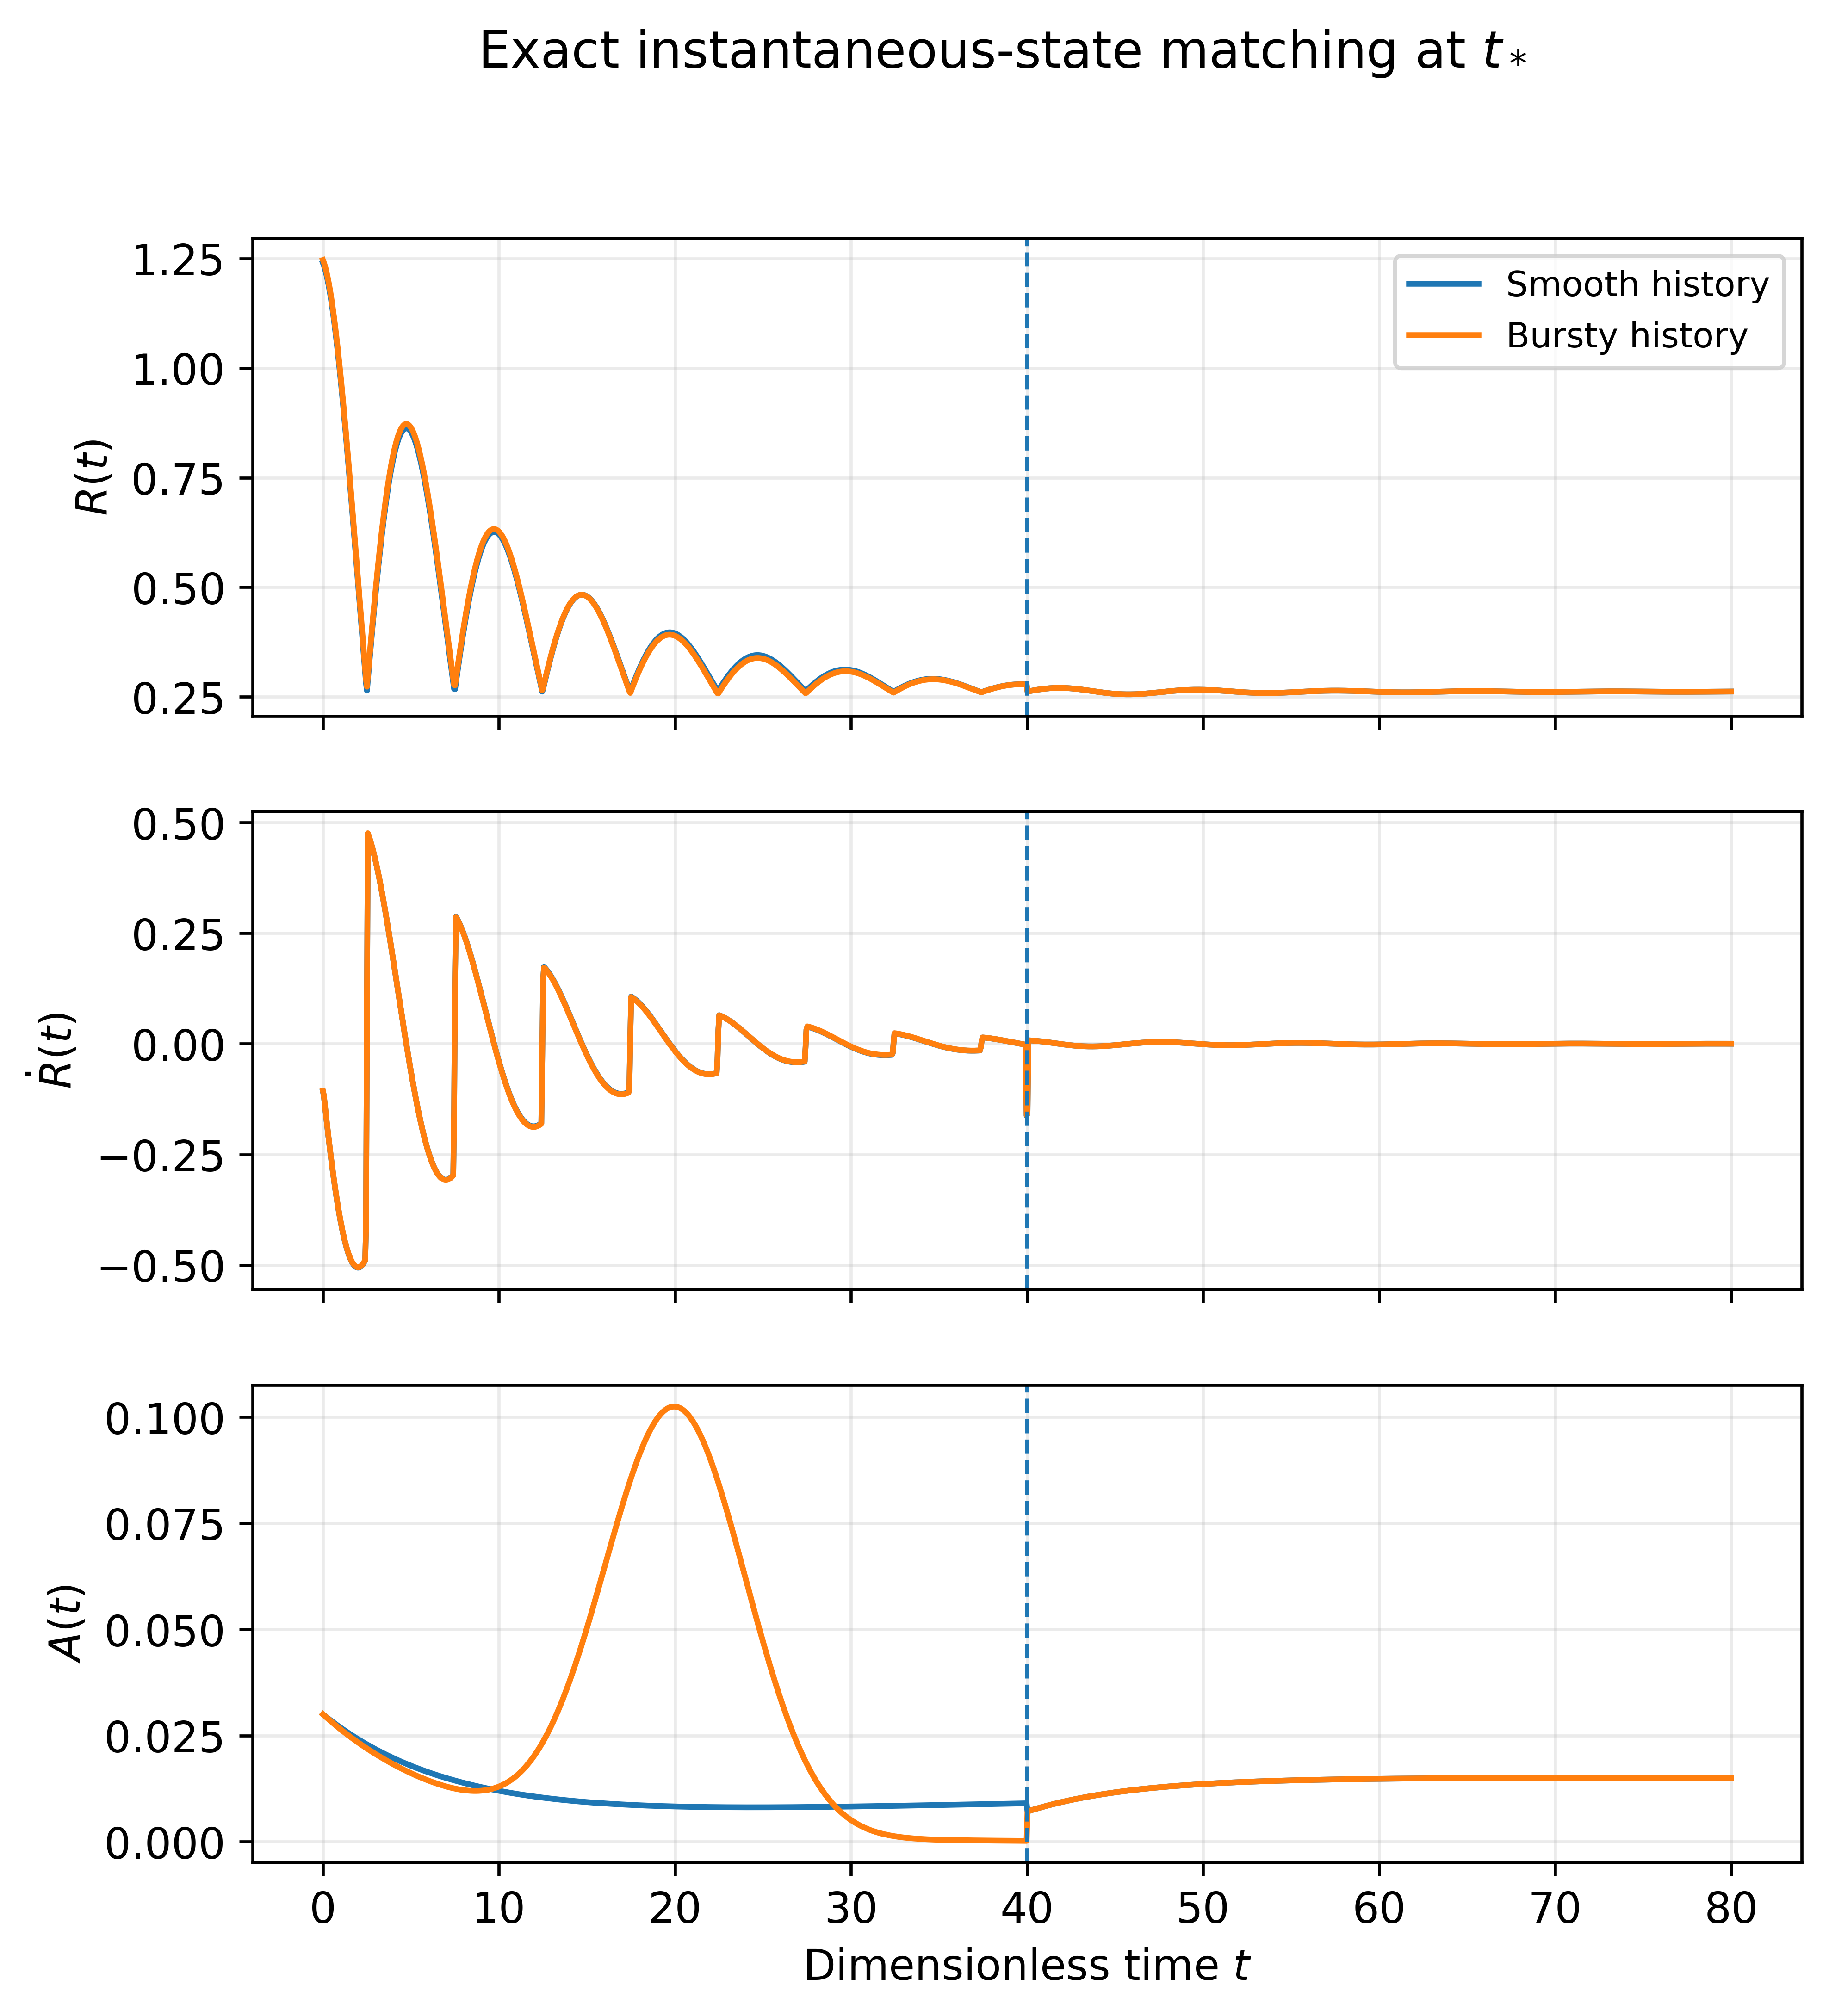
\includegraphics[width=\textwidth]{fig1_amplified_state_matching.png}
\caption{Exact instantaneous-state matching in the amplified-history fixed-scan toy model. The smooth and bursty histories are forced at \(t_\ast\) to share the same values of \(R\), \(\dot R\), and \(A\), while the retained memory coordinate is not reset.}
\label{fig:toy_state_matching}
\end{figure}

\begin{figure}[t]
\centering
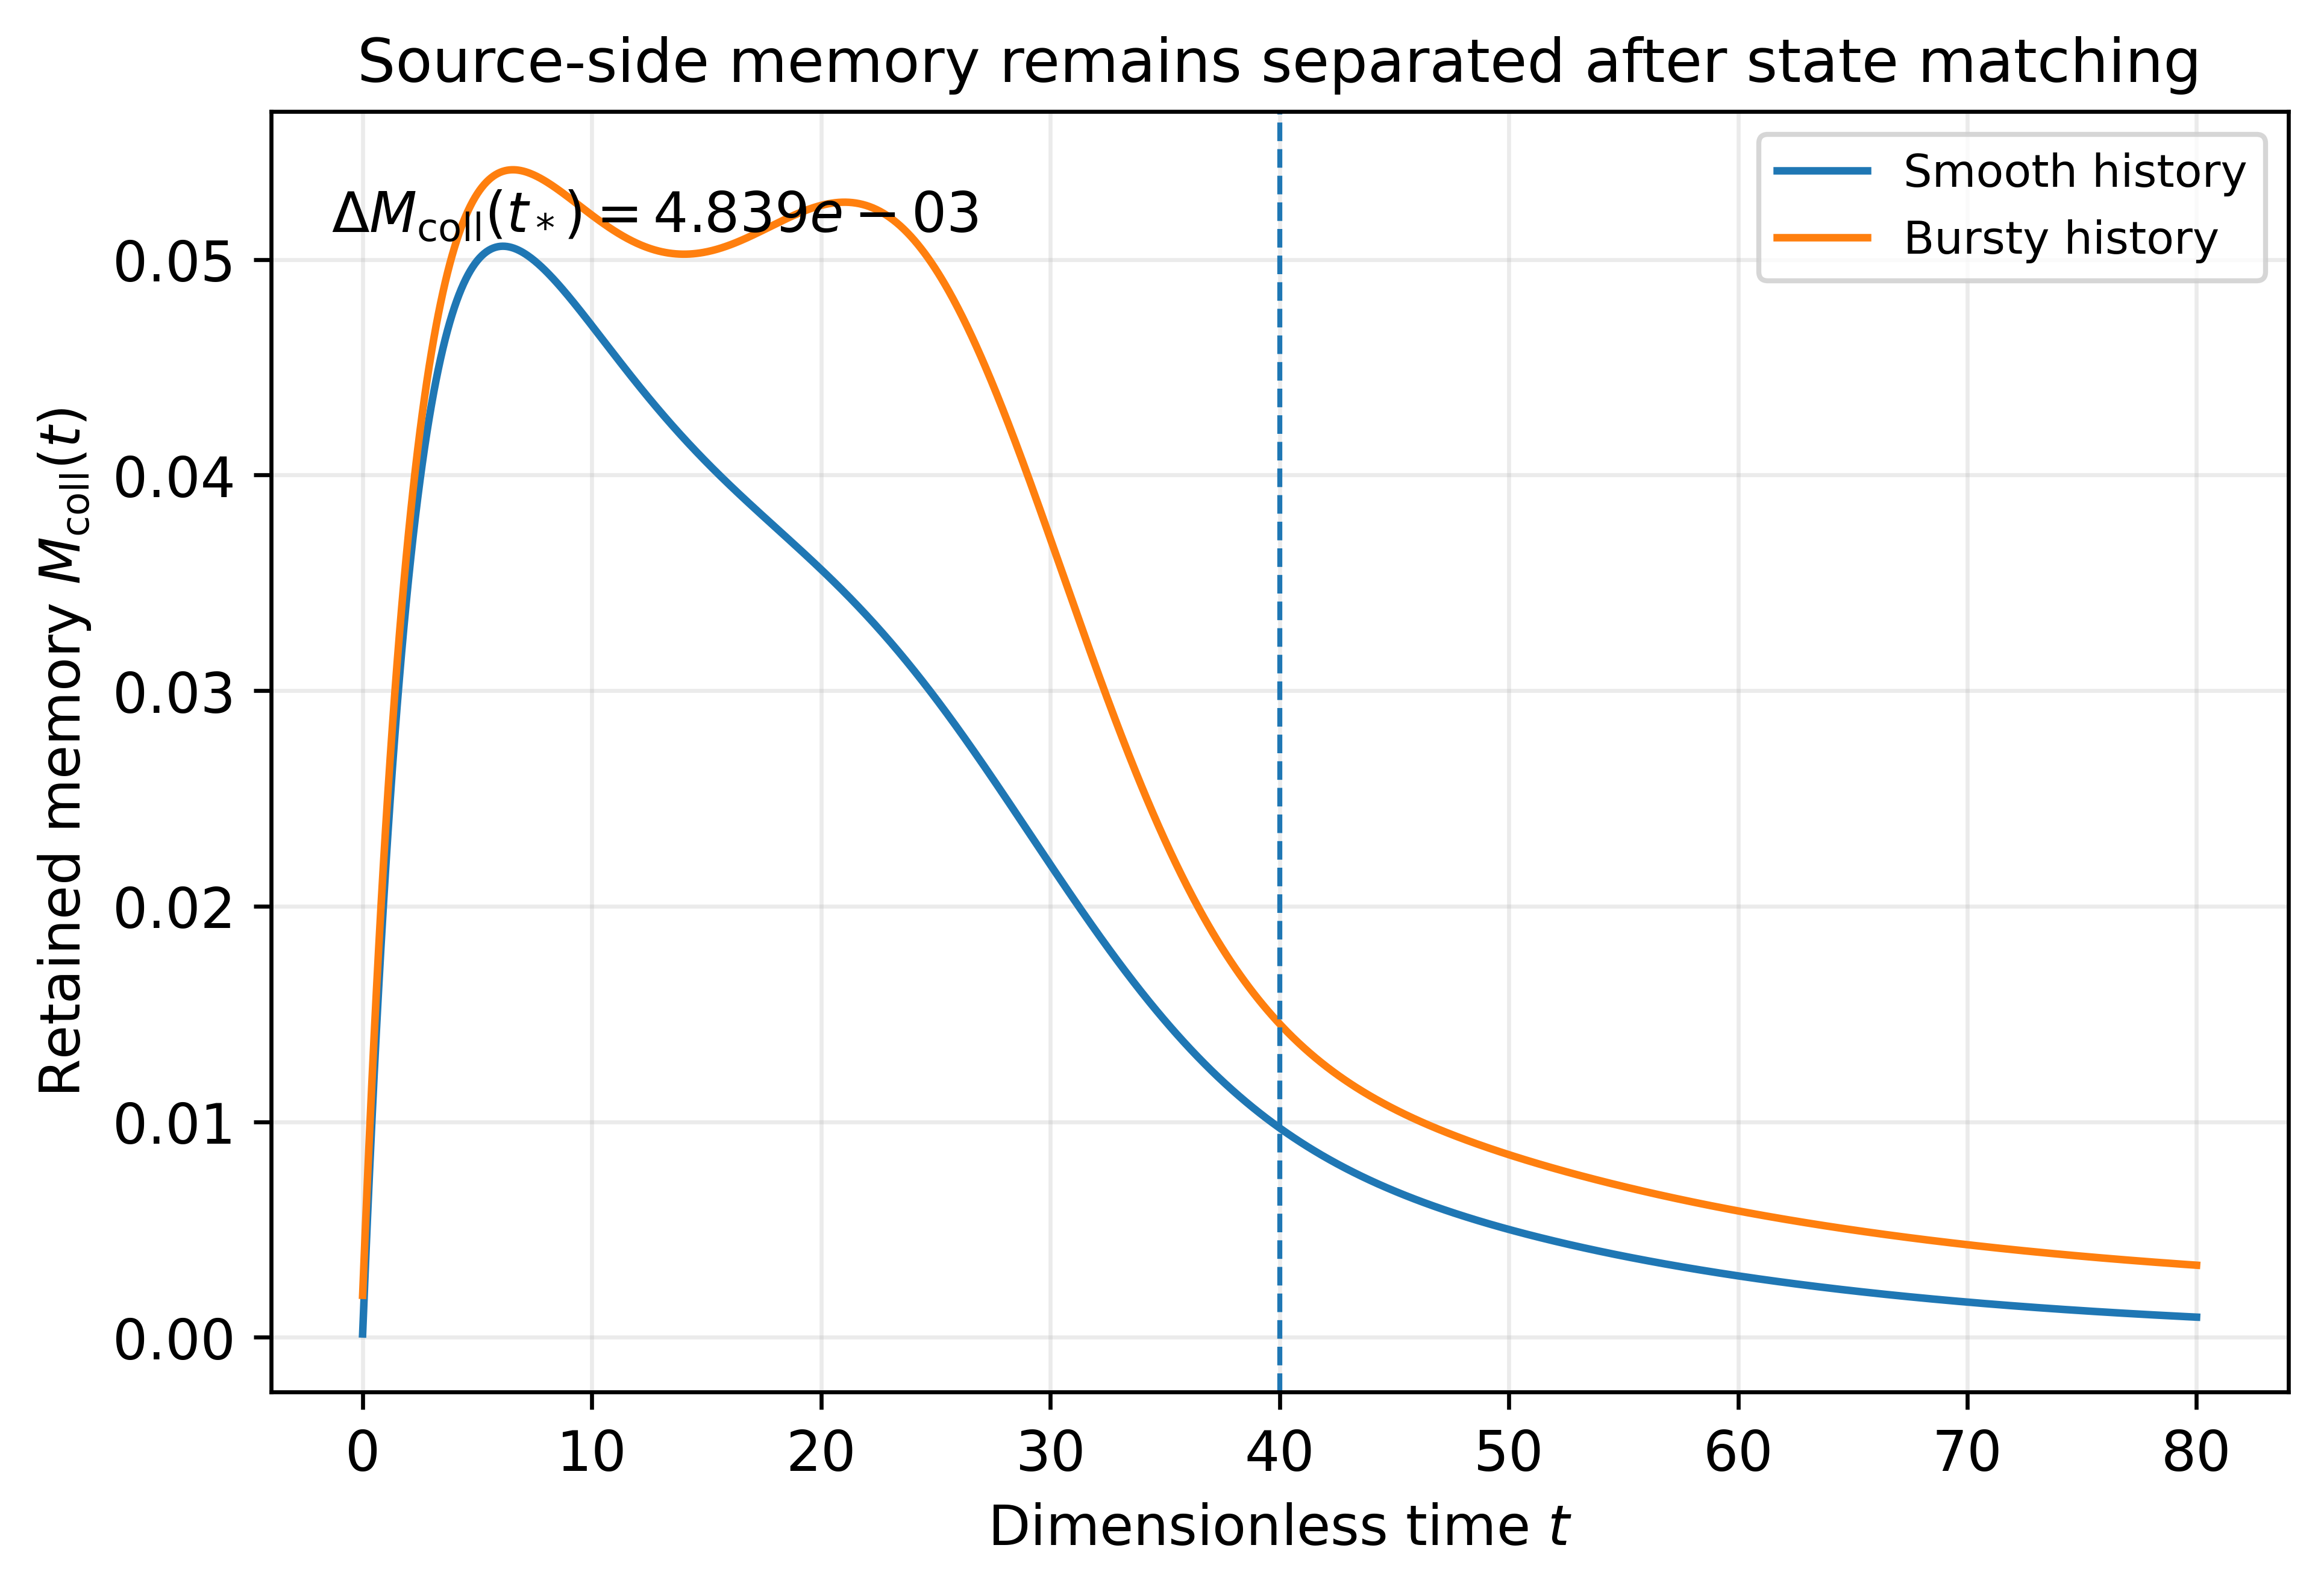
\includegraphics[width=0.92\textwidth]{fig2_amplified_memory_split.png}
\caption{Retained source-side memory separation after matched-state resetting. Although instantaneous variables are matched at \(t_\ast\), the two histories preserve \(\Delta M_{\rm coll}(t_\ast)=4.839\times10^{-3}\).}
\label{fig:toy_memory_split}
\end{figure}

\begin{figure}[t]
\centering
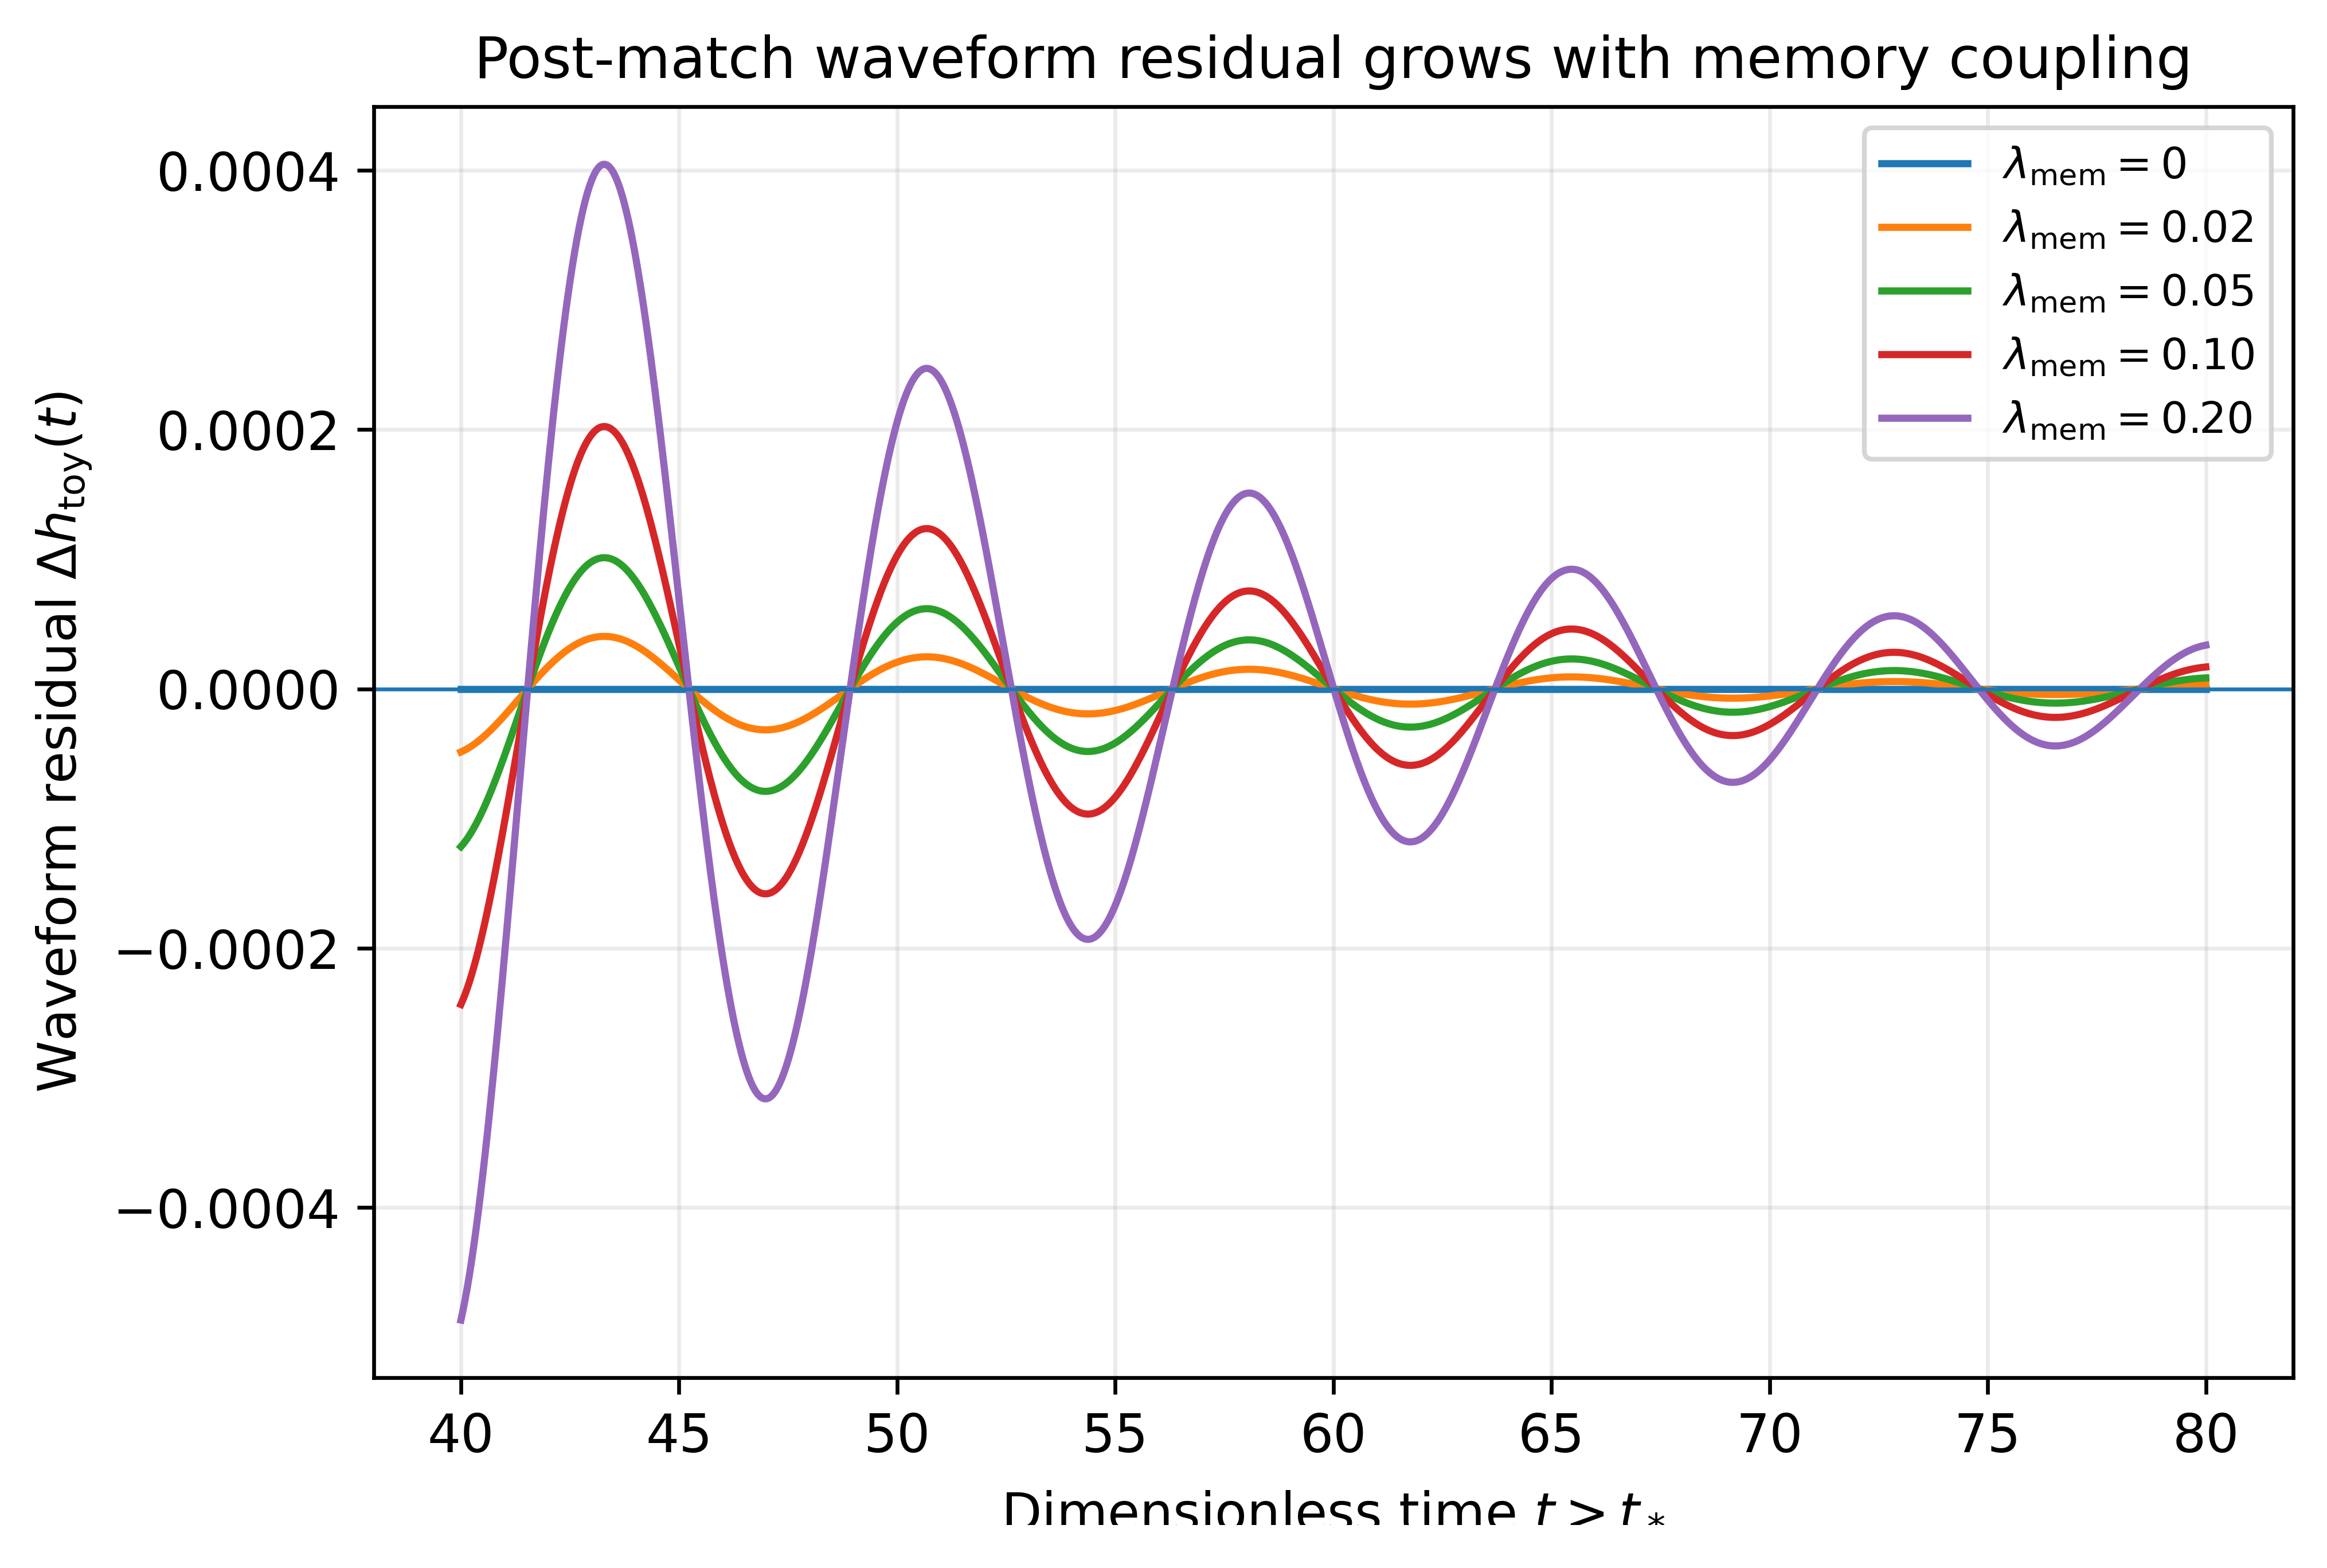
\includegraphics[width=0.92\textwidth]{fig3_amplified_waveform_residuals.png}
\caption{Post-match waveform residuals for the amplified-history fixed scan. The Markovian null remains near zero, while nonzero memory coupling produces structured residuals that increase with \(\lambda_{\rm mem}\).}
\label{fig:toy_waveform_residuals}
\end{figure}

\begin{figure}[t]
\centering
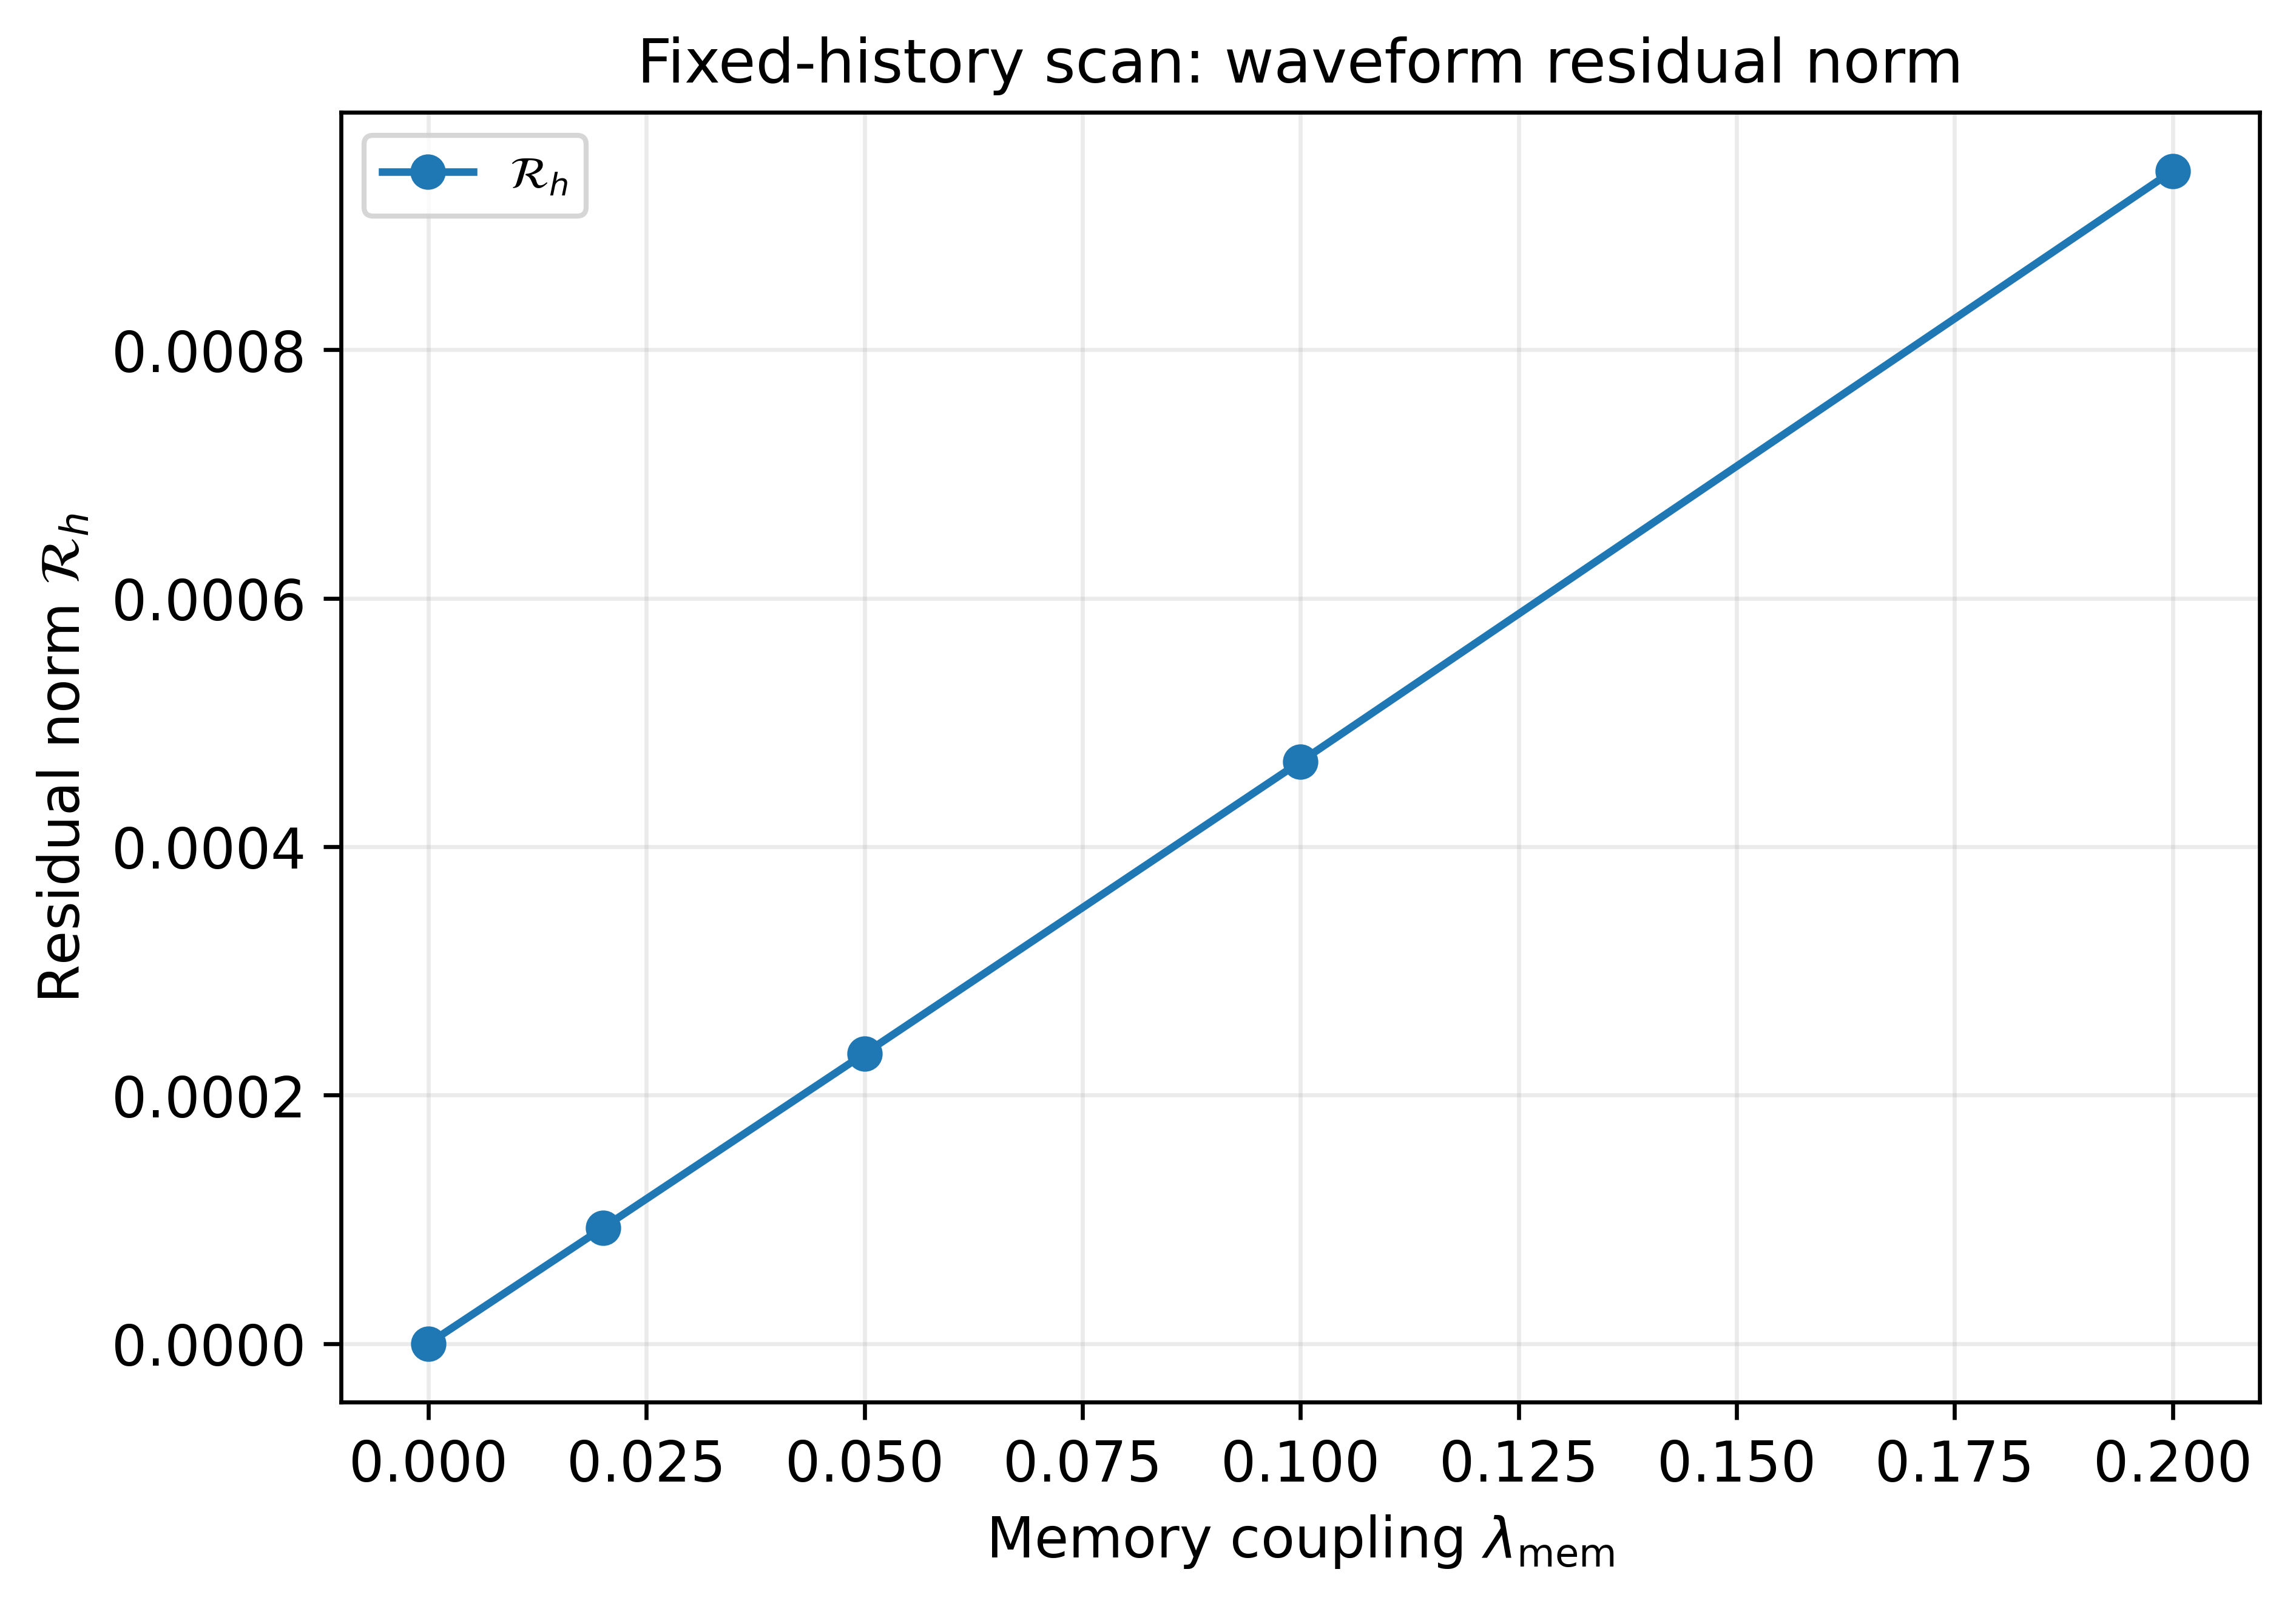
\includegraphics[width=0.82\textwidth]{fig4_lambda_scan_residual_norm.png}
\caption{Waveform residual norm as a function of memory-coupling strength. The retained memory contrast is held fixed across the scan, so the monotonic increase in \(\mathcal{R}_h\) reflects the dynamical effect of source-memory coupling.}
\label{fig:toy_lambda_scan}
\end{figure}

A conservative baseline run was also retained as a robustness check. In that run, \(\Delta M_{\rm coll}(t_\ast)=2.35\times10^{-5}\), \(\mathcal{R}_h(\lambda_{\rm mem}=0)=2.14\times10^{-10}\), and \(\mathcal{R}_h(\lambda_{\rm mem}=0.20)=4.27\times10^{-6}\). The qualitative effect is the same, but the amplified run is used as the primary demonstration because it avoids relying on a marginal memory contrast.

\section{Synthetic Detector and Network Validation}
\label{sec:detector_validation}

The detector tests are deliberately synthetic. They do not constitute a LIGO/Virgo/KAGRA sensitivity forecast. Their purpose is to ask whether the memory-completed residual behaves as a distinguishable waveform component under colored noise, detector-response projection, and network combination.

\subsection{Single-detector colored-noise injection}

The amplified-history residual with \(\lambda_{\rm mem}=0.20\) was normalized to a target matched-filter signal-to-noise ratio of 12 and injected into 200 independent colored-noise realizations. The template bank consisted of \(\lambda_{\rm mem}\in\{0.00,0.02,0.05,0.10,0.20\}\). The memory-free null was strongly rejected. The injected memory template recovered \(11.9998\pm0.0156\), while the Markovian-null template recovered \(0.00095\pm0.01875\). The mean memory-minus-null contrast was \(11.9989\pm0.0239\).

The same test exposes an important limitation. All nonzero memory templates recovered high scores, with mean values \(11.9667\), \(11.9769\), \(11.9897\), and \(11.9998\) for \(\lambda_{\rm mem}=0.02,0.05,0.10,0.20\), respectively. The nonzero templates are therefore highly degenerate in shape. The mean overlap among nonzero templates is \(0.998939\), with a minimum of \(0.997238\), whereas the maximum overlap between the null and any memory-on template is only \(0.000723\). This geometry indicates a nearly flat nonzero-memory direction in the present template family: even a weak memory template with \(\lambda_{\rm mem}=0.02\) pulls a strong \(\lambda_{\rm inj}=0.20\) injection out of the null space, but it does not sharply localize the injected coupling. The present detector-level toy test therefore supports memory-on versus memory-off distinguishability, not precision estimation of \(\lambda_{\rm mem}\). This flat direction is one reason the second phase lifts the scalar memory coordinate into multidimensional \(3+1\) variables: richer field structure is needed before parameter resolution can be treated as a serious inference target.

\begin{figure}[t]
\centering
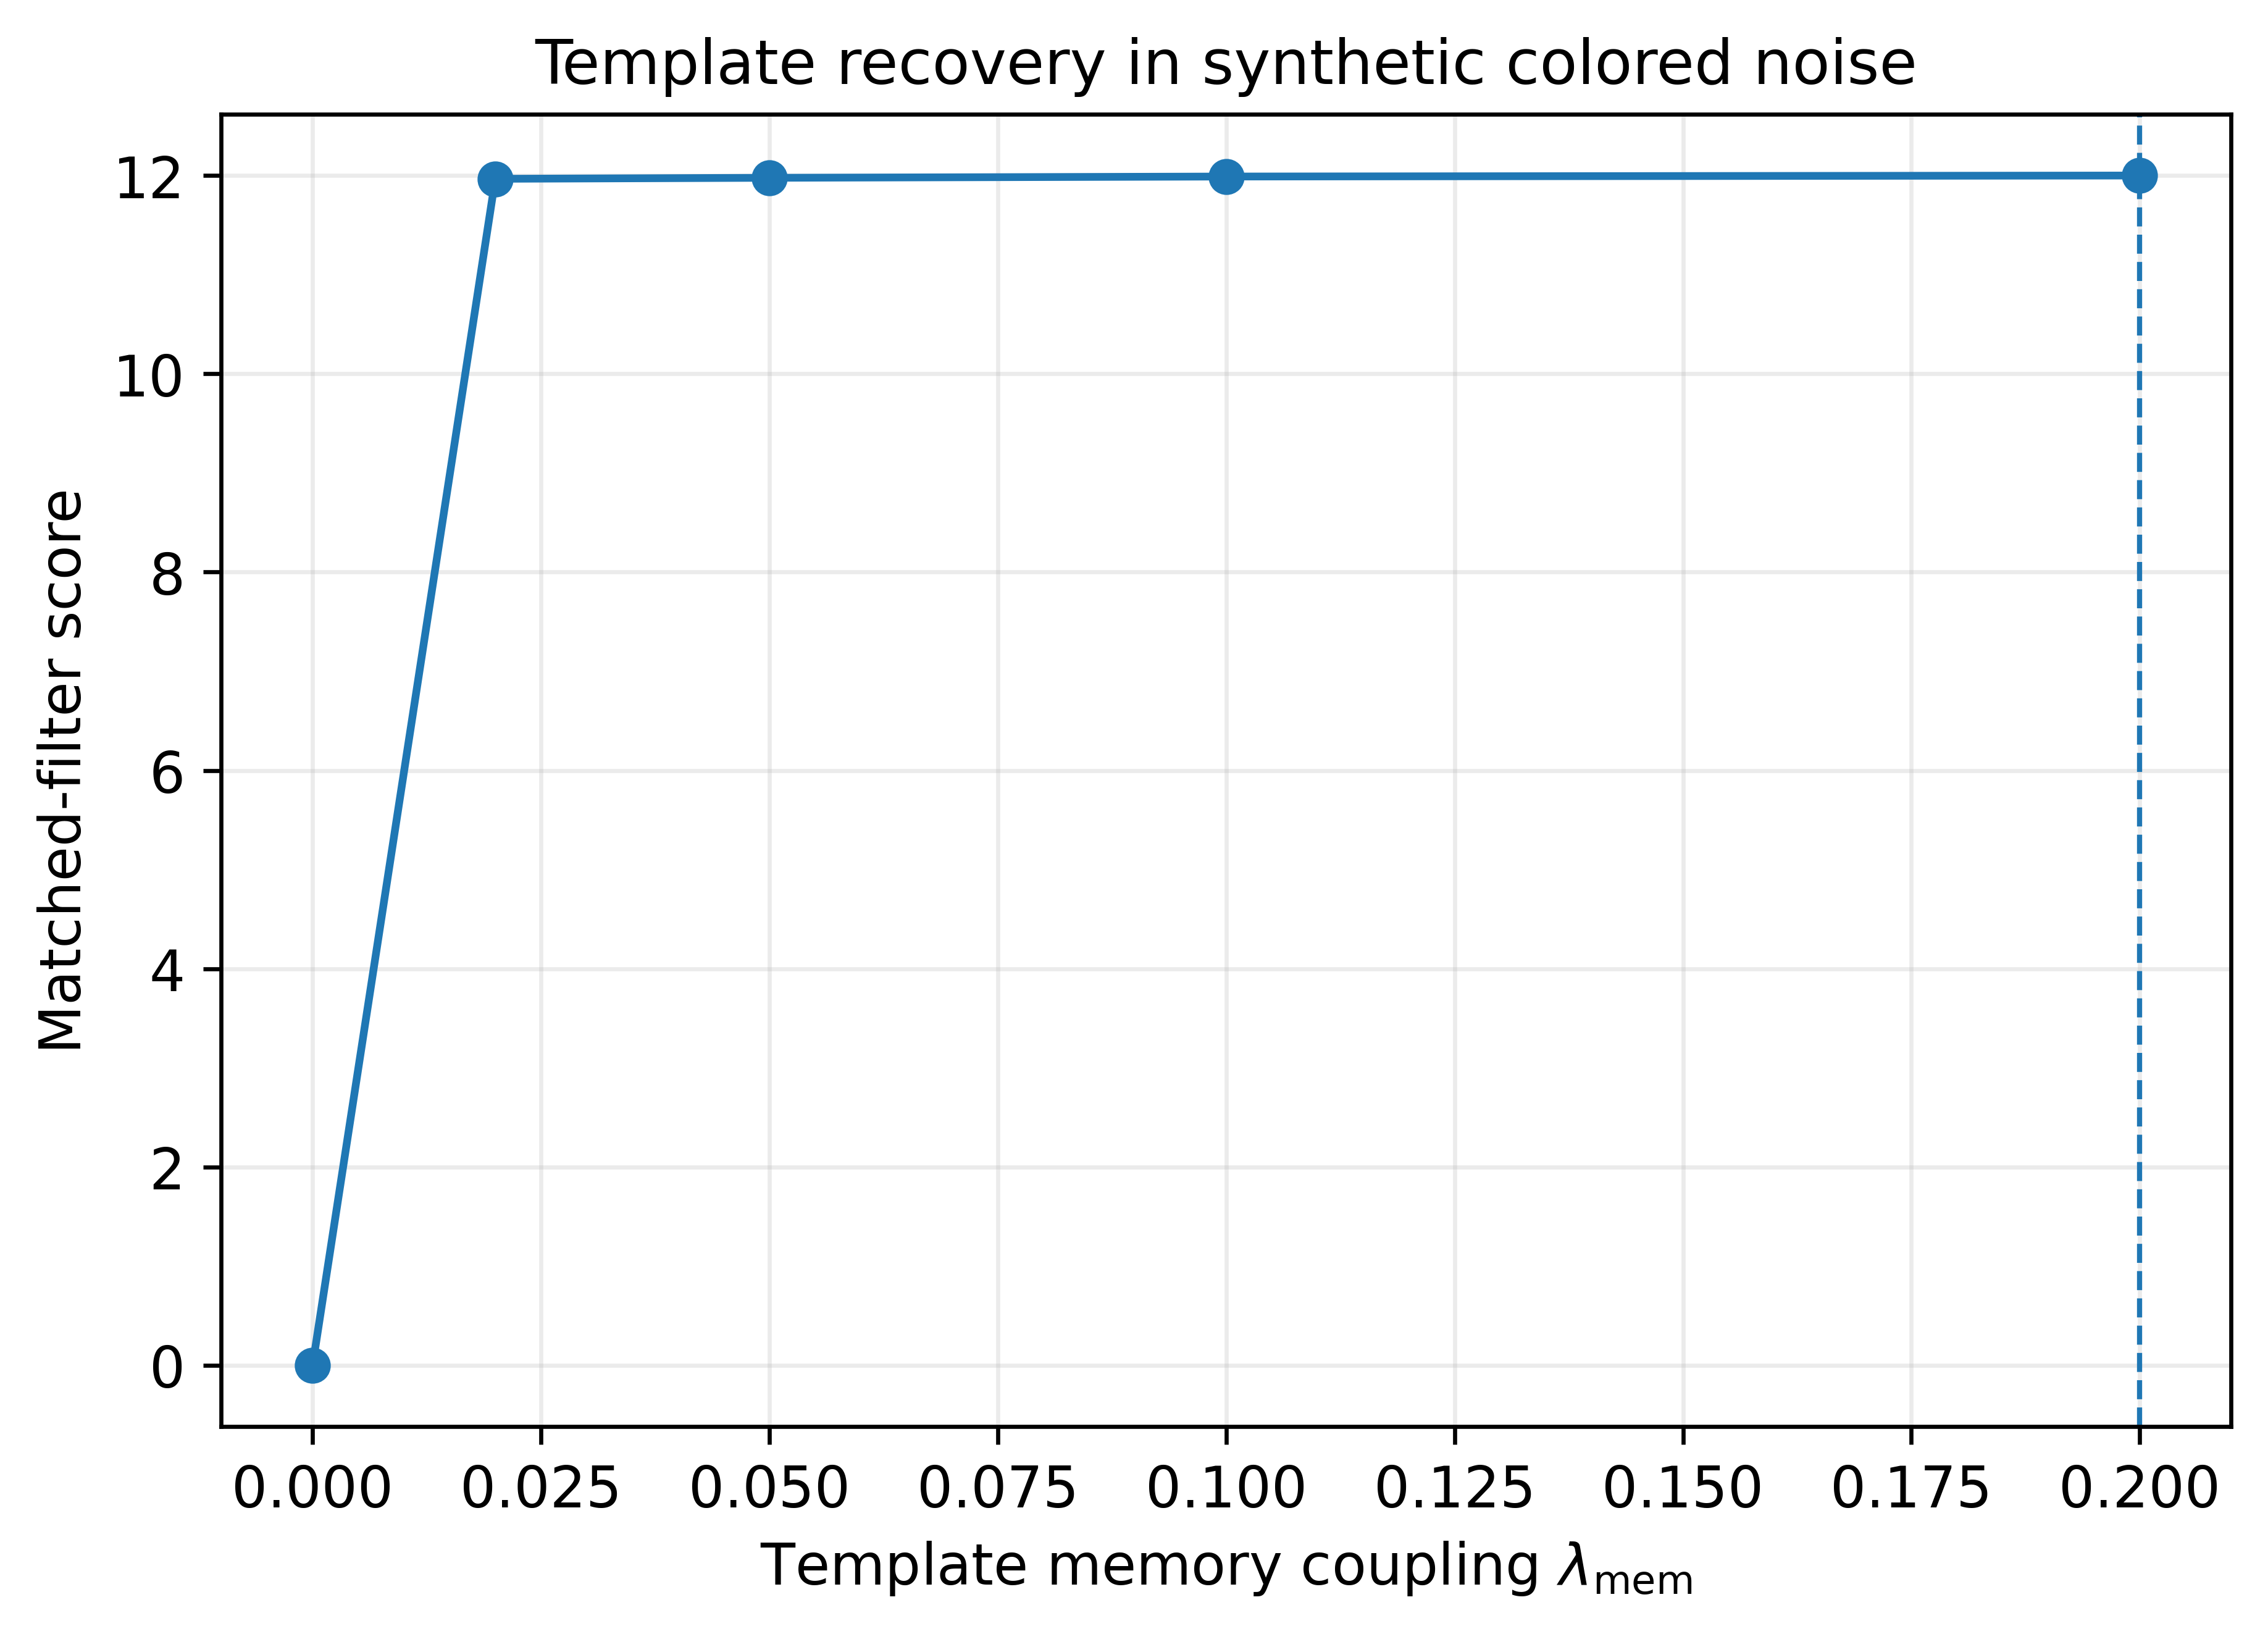
\includegraphics[width=0.86\textwidth]{synthetic_detector_template_snr_scan.png}
\caption{Single-detector synthetic colored-noise recovery. The injected \(\lambda_{\rm mem}=0.20\) memory waveform is strongly separated from the Markovian null, while nonzero memory templates remain nearly degenerate.}
\label{fig:single_detector_snr_scan}
\end{figure}

\begin{figure}[t]
\centering
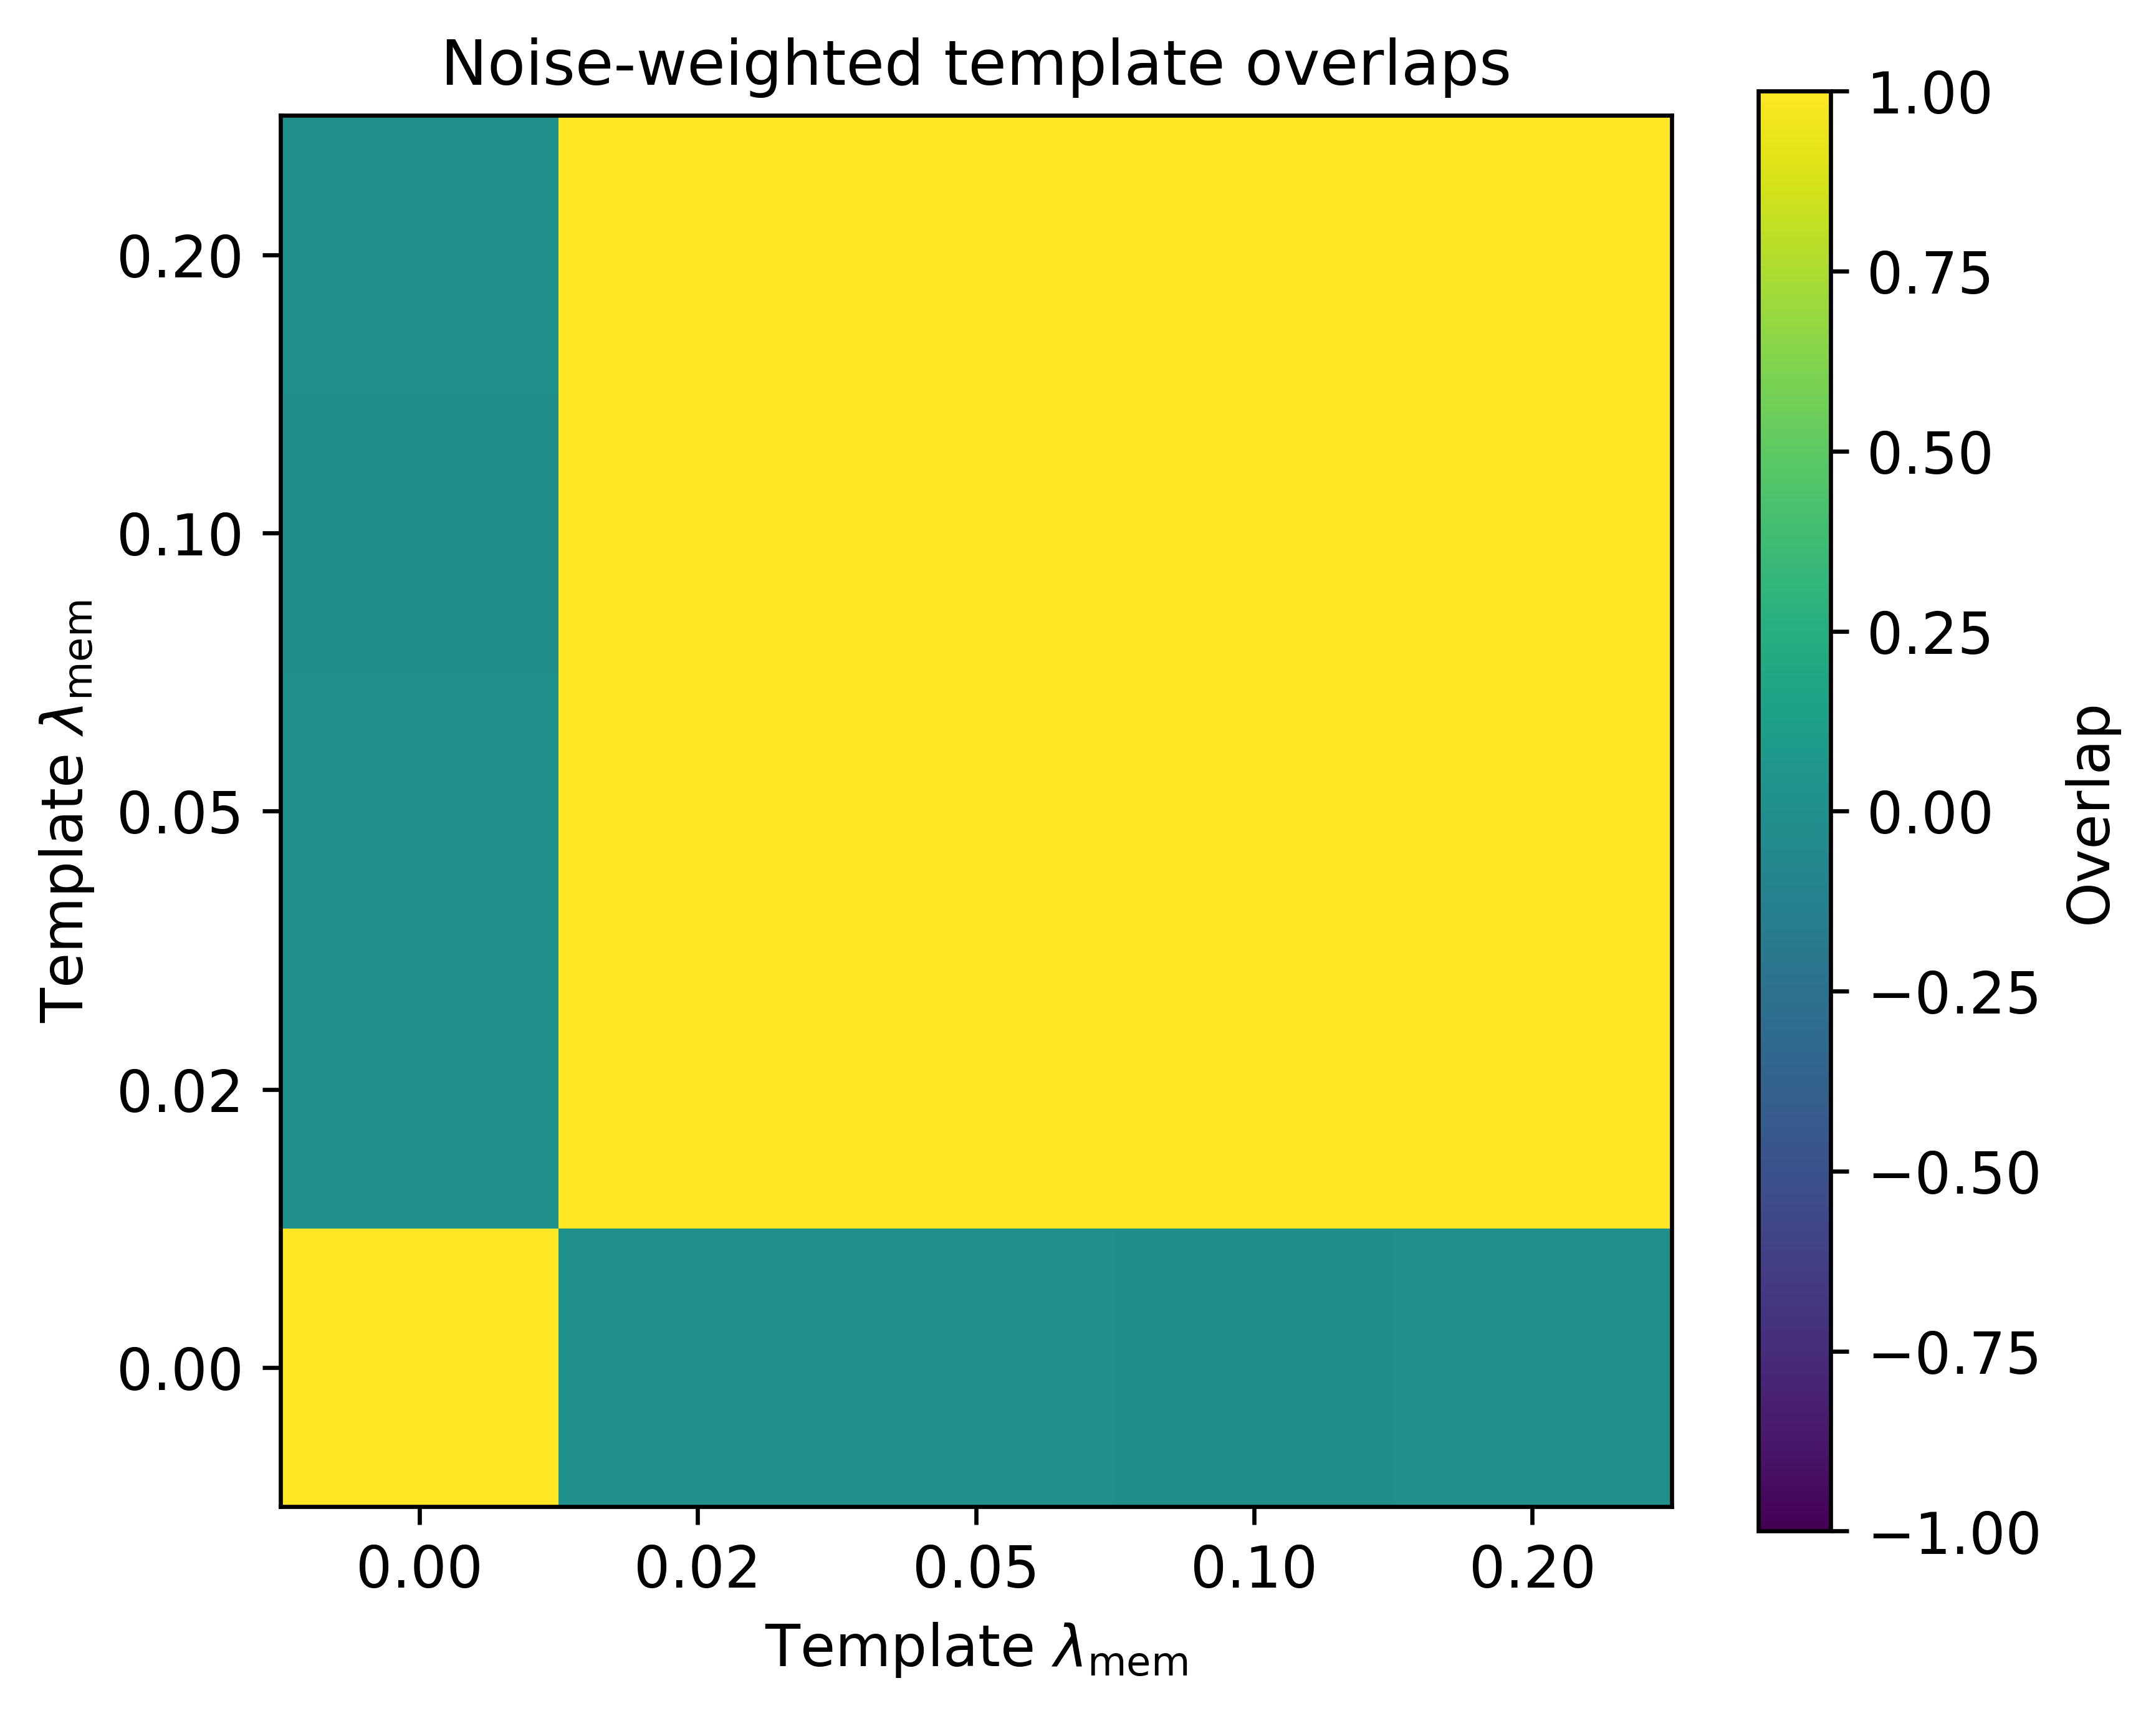
\includegraphics[width=0.72\textwidth]{synthetic_detector_template_overlap_matrix.png}
\caption{Noise-weighted template overlaps in the synthetic single-detector test. Nonzero memory templates are highly correlated with each other, but nearly orthogonal to the Markovian null.}
\label{fig:single_detector_overlap}
\end{figure}

\subsection{Three-detector synthetic network}

A three-detector H1/L1/V1-like synthetic network was then constructed using controlled antenna-response coefficients, detector-specific time delays, and different colored-noise scales. The coefficients are not official detector response tensors. They are used to test network architecture under a transparent toy setup.

The injected signal was normalized to \(\rho_{\rm net}=15\), with optimal detector contributions \(\rho_{\rm H1}=10.666\), \(\rho_{\rm L1}=9.927\), and \(\rho_{\rm V1}=3.561\). Across 200 colored-noise trials, the memory template recovered \(15.0002\pm0.0165\), while the Markovian null recovered \(0.0415\pm0.0120\) in the V1-glitch scenario. The memory-minus-null contrast was \(14.9587\). A no-glitch comparison recovered \(15.0002\pm0.0165\) for the memory template and \(0.0250\pm0.0109\) for the null template. The V1 transient therefore leaves the true memory-template recovery unchanged but raises the null-template floor by approximately \(65\%\), from \(0.0250\) to \(0.0415\). This updrift is small in absolute terms but diagnostically useful: non-Gaussian transient power leaks more visibly into the oversimplified null channel than into the correctly structured memory template. Thus, under this synthetic architecture, the memory-completed signal remains strongly distinguishable from the memory-free null after time delays, detector-response projections, colored noise, and a weak third-detector channel are included.

\begin{table}[t]
\centering
\caption{Synthetic detector contributions in the three-detector network injection. The coefficients are controlled toy antenna-response factors, not official H1/L1/V1 response tensors.}
\begin{tabular}{lccccc}
\toprule
Detector & Delay [ms] & Delay [samples] & \(F_+\) & \(F_\times\) & Optimal SNR \\
\midrule
H1 & 0.0 & 0 & 0.70 & 0.20 & 10.666 \\
L1 & 7.1 & 11 & -0.62 & 0.25 & 9.927 \\
V1 & -14.3 & -23 & 0.28 & -0.36 & 3.561 \\
\bottomrule
\end{tabular}
\label{tab:network_detector_contributions}
\end{table}

\begin{table}[t]
\centering
\caption{Synthetic network recovery with and without a V1-channel sine-Gaussian glitch. The memory-template recovery is stable in both cases, while the Markovian-null response remains strongly suppressed.}
\begin{tabular}{lcccc}
\toprule
Scenario & \(\rho_{\rm mem}\) & \(\rho_{\rm null}\) & \(\Delta\rho\) & \(E_C/E_I\) \\
\midrule
No glitch & \(15.0002\pm0.0165\) & \(0.0250\pm0.0109\) & 14.9752 & \(2.5929\pm0.0017\) \\
V1 glitch & \(15.0002\pm0.0165\) & \(0.0415\pm0.0120\) & 14.9587 & \(2.5929\pm0.0017\) \\
\bottomrule
\end{tabular}
\label{tab:network_glitch_comparison}
\end{table}

The coherence diagnostic \(E_C/E_I\) is intentionally treated as a toy statistic, not a calibrated false-alarm measure. In this implementation it is insensitive to the injected V1 glitch because the glitch is not strongly aligned with the memory template. The glitch test is therefore interpreted as a recovery-stability check, not as a full glitch-rejection analysis.

\begin{figure}[t]
\centering
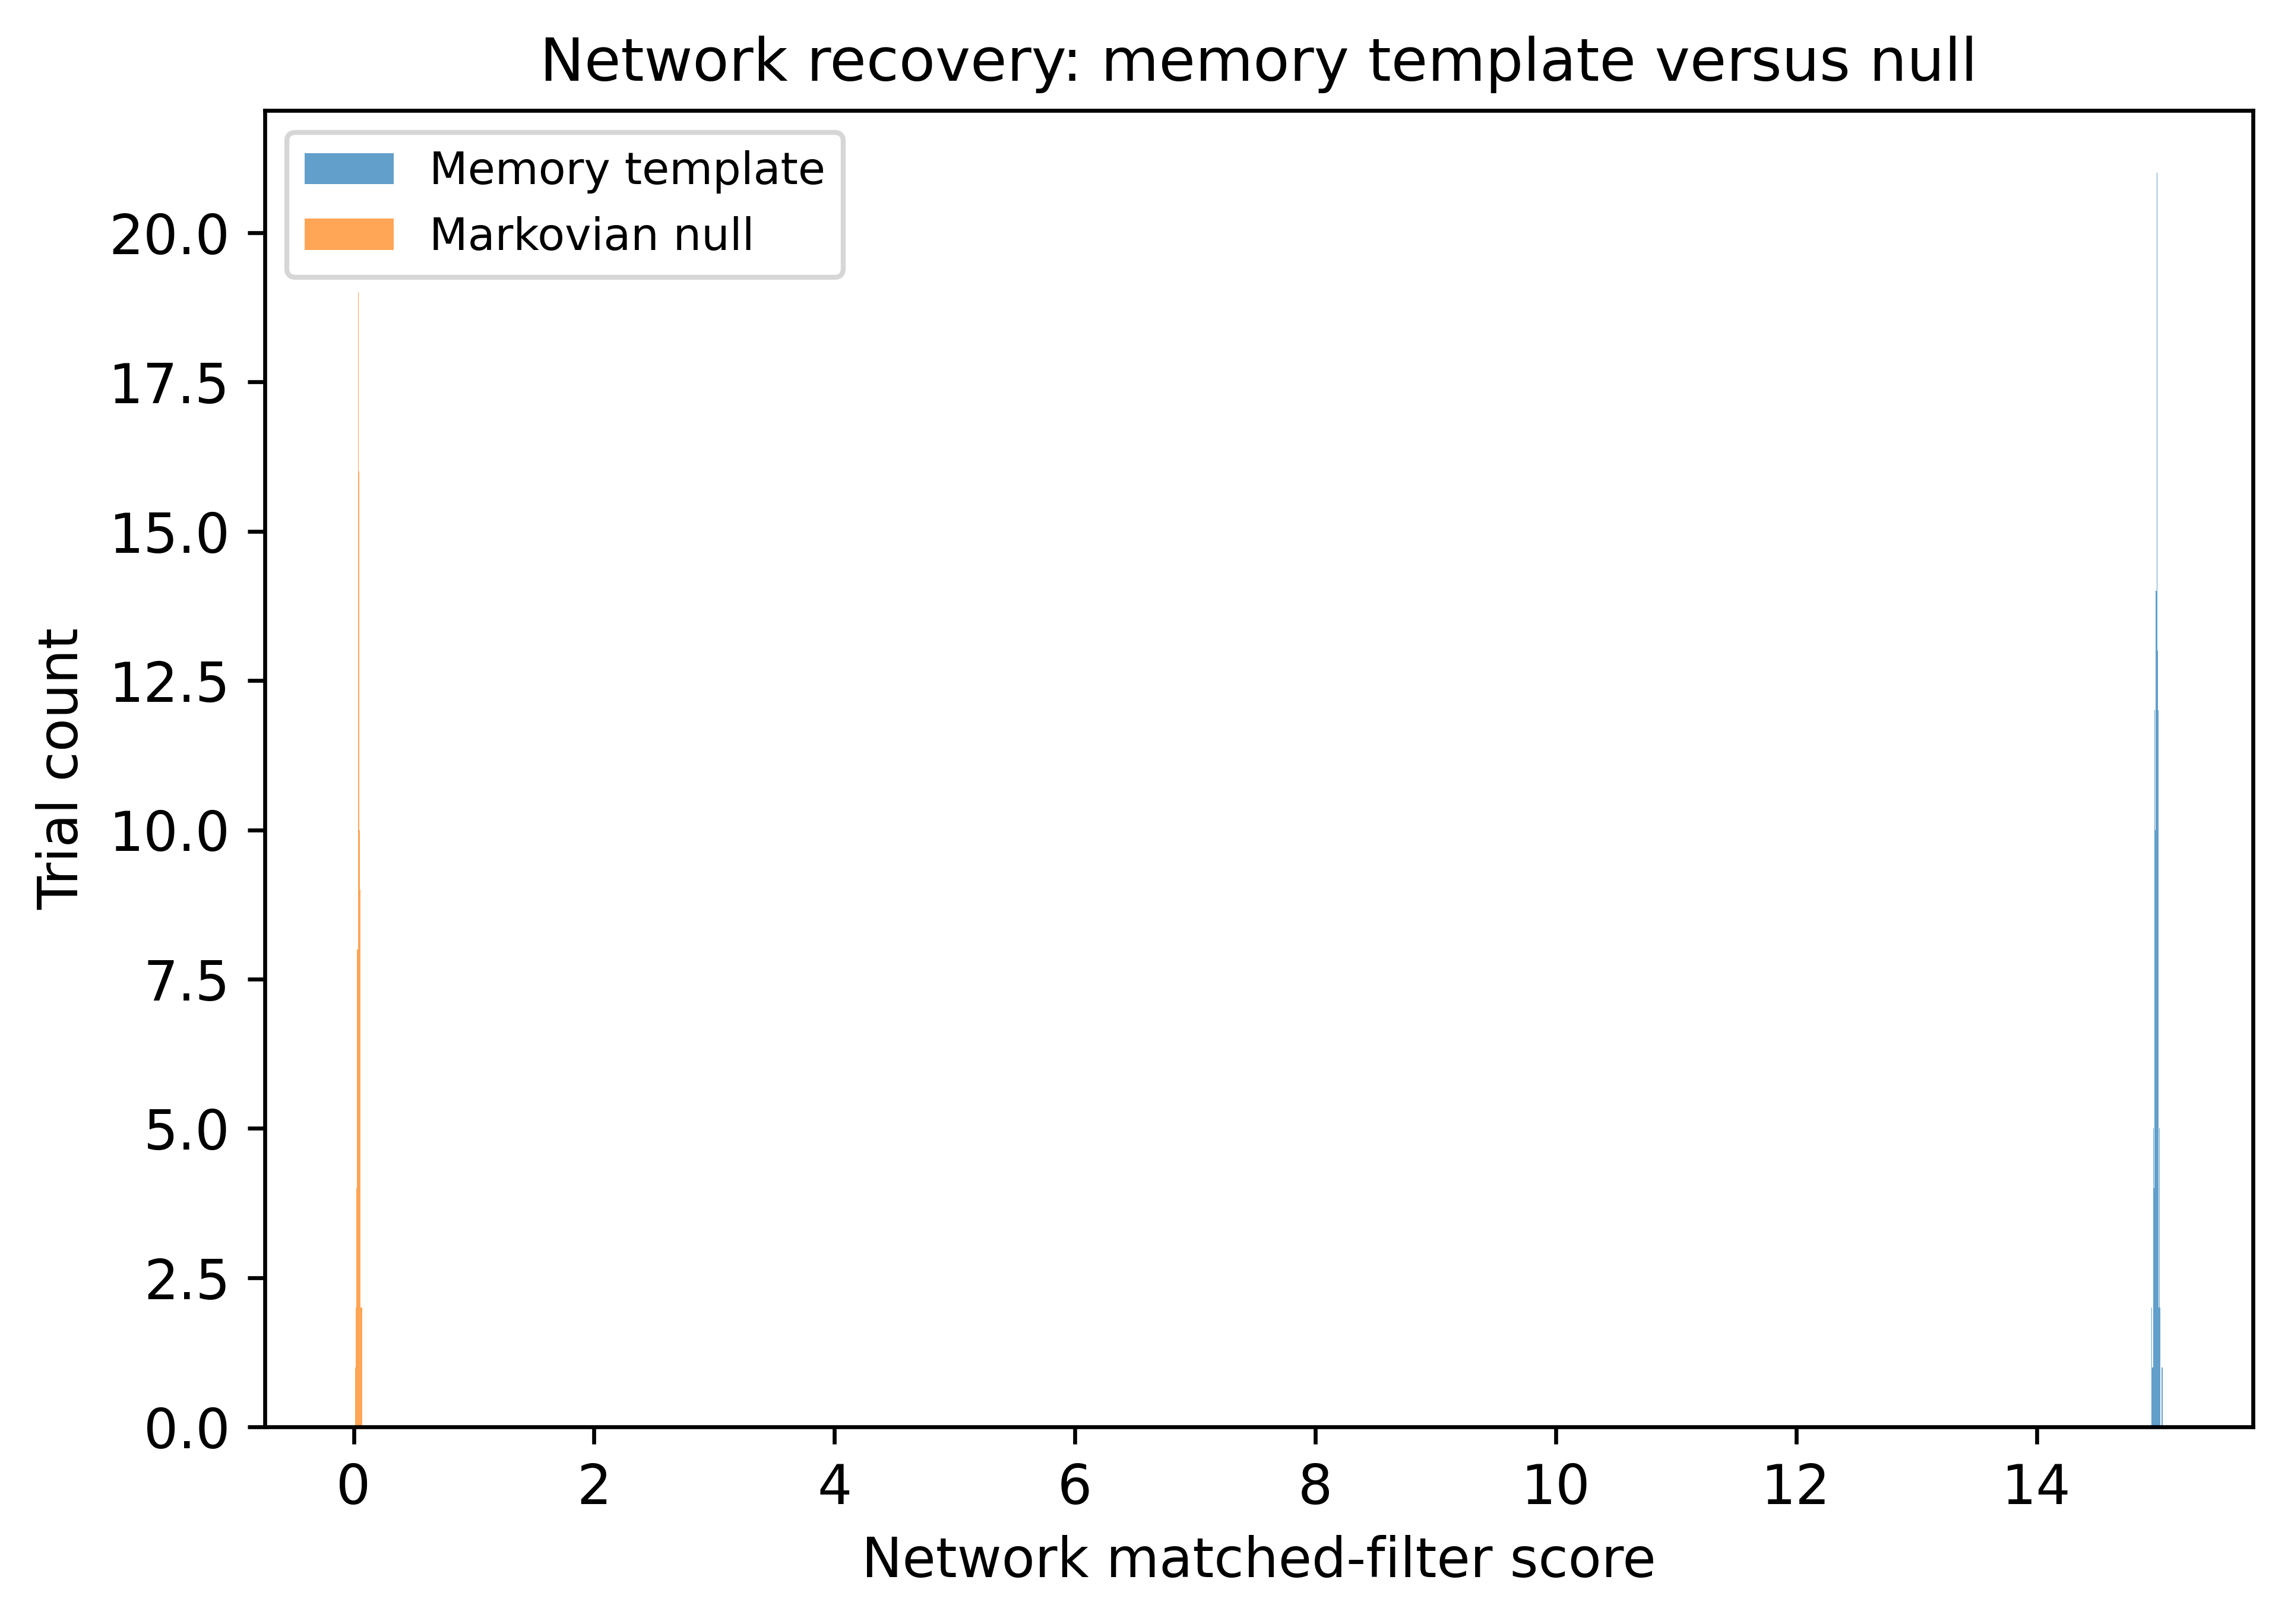
\includegraphics[width=0.86\textwidth]{network_memory_vs_null_hist.png}
\caption{Three-detector synthetic network recovery. The memory template recovers the injected network signal, while the Markovian null remains strongly suppressed.}
\label{fig:network_memory_null}
\end{figure}

\subsection{Network SNR-threshold scan}

A no-glitch network SNR-threshold scan was performed for injected target values \(\rho_{\rm net}\in\{3,5,8,10,12,15\}\). Across 200 colored-noise trials at each grid point, the memory template recovered the injected network score nearly exactly, while the null template remained near \(0.025\). At the lowest tested injection strength, \(\rho_{\rm net}=3\), the memory template recovered \(3.0003\pm0.0165\), whereas the null recovered \(0.0251\pm0.0110\). The corresponding individual optimal detector contributions were \(\rho_{\rm H1}=2.13\), \(\rho_{\rm L1}=1.99\), and \(\rho_{\rm V1}=0.71\). In this toy architecture, each individual channel is therefore below a plausible standalone trigger scale, while the coherent network still recovers the path-dependent signal. At \(\rho_{\rm net}=15\), the recovered memory and null scores were \(15.0002\pm0.0165\) and \(0.0250\pm0.0109\), respectively. This indicates memory-on versus memory-off separability down to the lowest tested network SNR under the adopted synthetic-noise and projection assumptions.

\begin{table}[t]
\centering
\caption{Synthetic network SNR-threshold scan. The memory-completed waveform remains distinguishable from the Markovian-null template across the tested injected network-SNR range. Each row summarizes 200 colored-noise trials.}
\begin{tabular}{ccccc}
\toprule
Injected \(\rho_{\rm net}\) & Recovered memory score & Recovered null score & \(\Delta\rho\) & \(E_C/E_I\) \\
\midrule
3  & \(3.0003\pm0.0165\)  & \(0.0251\pm0.0110\) & 2.9753  & \(2.5921\pm0.0083\) \\
5  & \(5.0003\pm0.0165\)  & \(0.0251\pm0.0110\) & 4.9752  & \(2.5925\pm0.0050\) \\
8  & \(8.0003\pm0.0165\)  & \(0.0250\pm0.0109\) & 7.9752  & \(2.5927\pm0.0031\) \\
10 & \(10.0003\pm0.0165\) & \(0.0250\pm0.0109\) & 9.9752  & \(2.5928\pm0.0025\) \\
12 & \(12.0003\pm0.0165\) & \(0.0250\pm0.0109\) & 11.9752 & \(2.5928\pm0.0021\) \\
15 & \(15.0002\pm0.0165\) & \(0.0250\pm0.0109\) & 14.9752 & \(2.5929\pm0.0017\) \\
\bottomrule
\end{tabular}
\label{tab:network_snr_threshold_scan}
\end{table}

\begin{figure}[t]
\centering
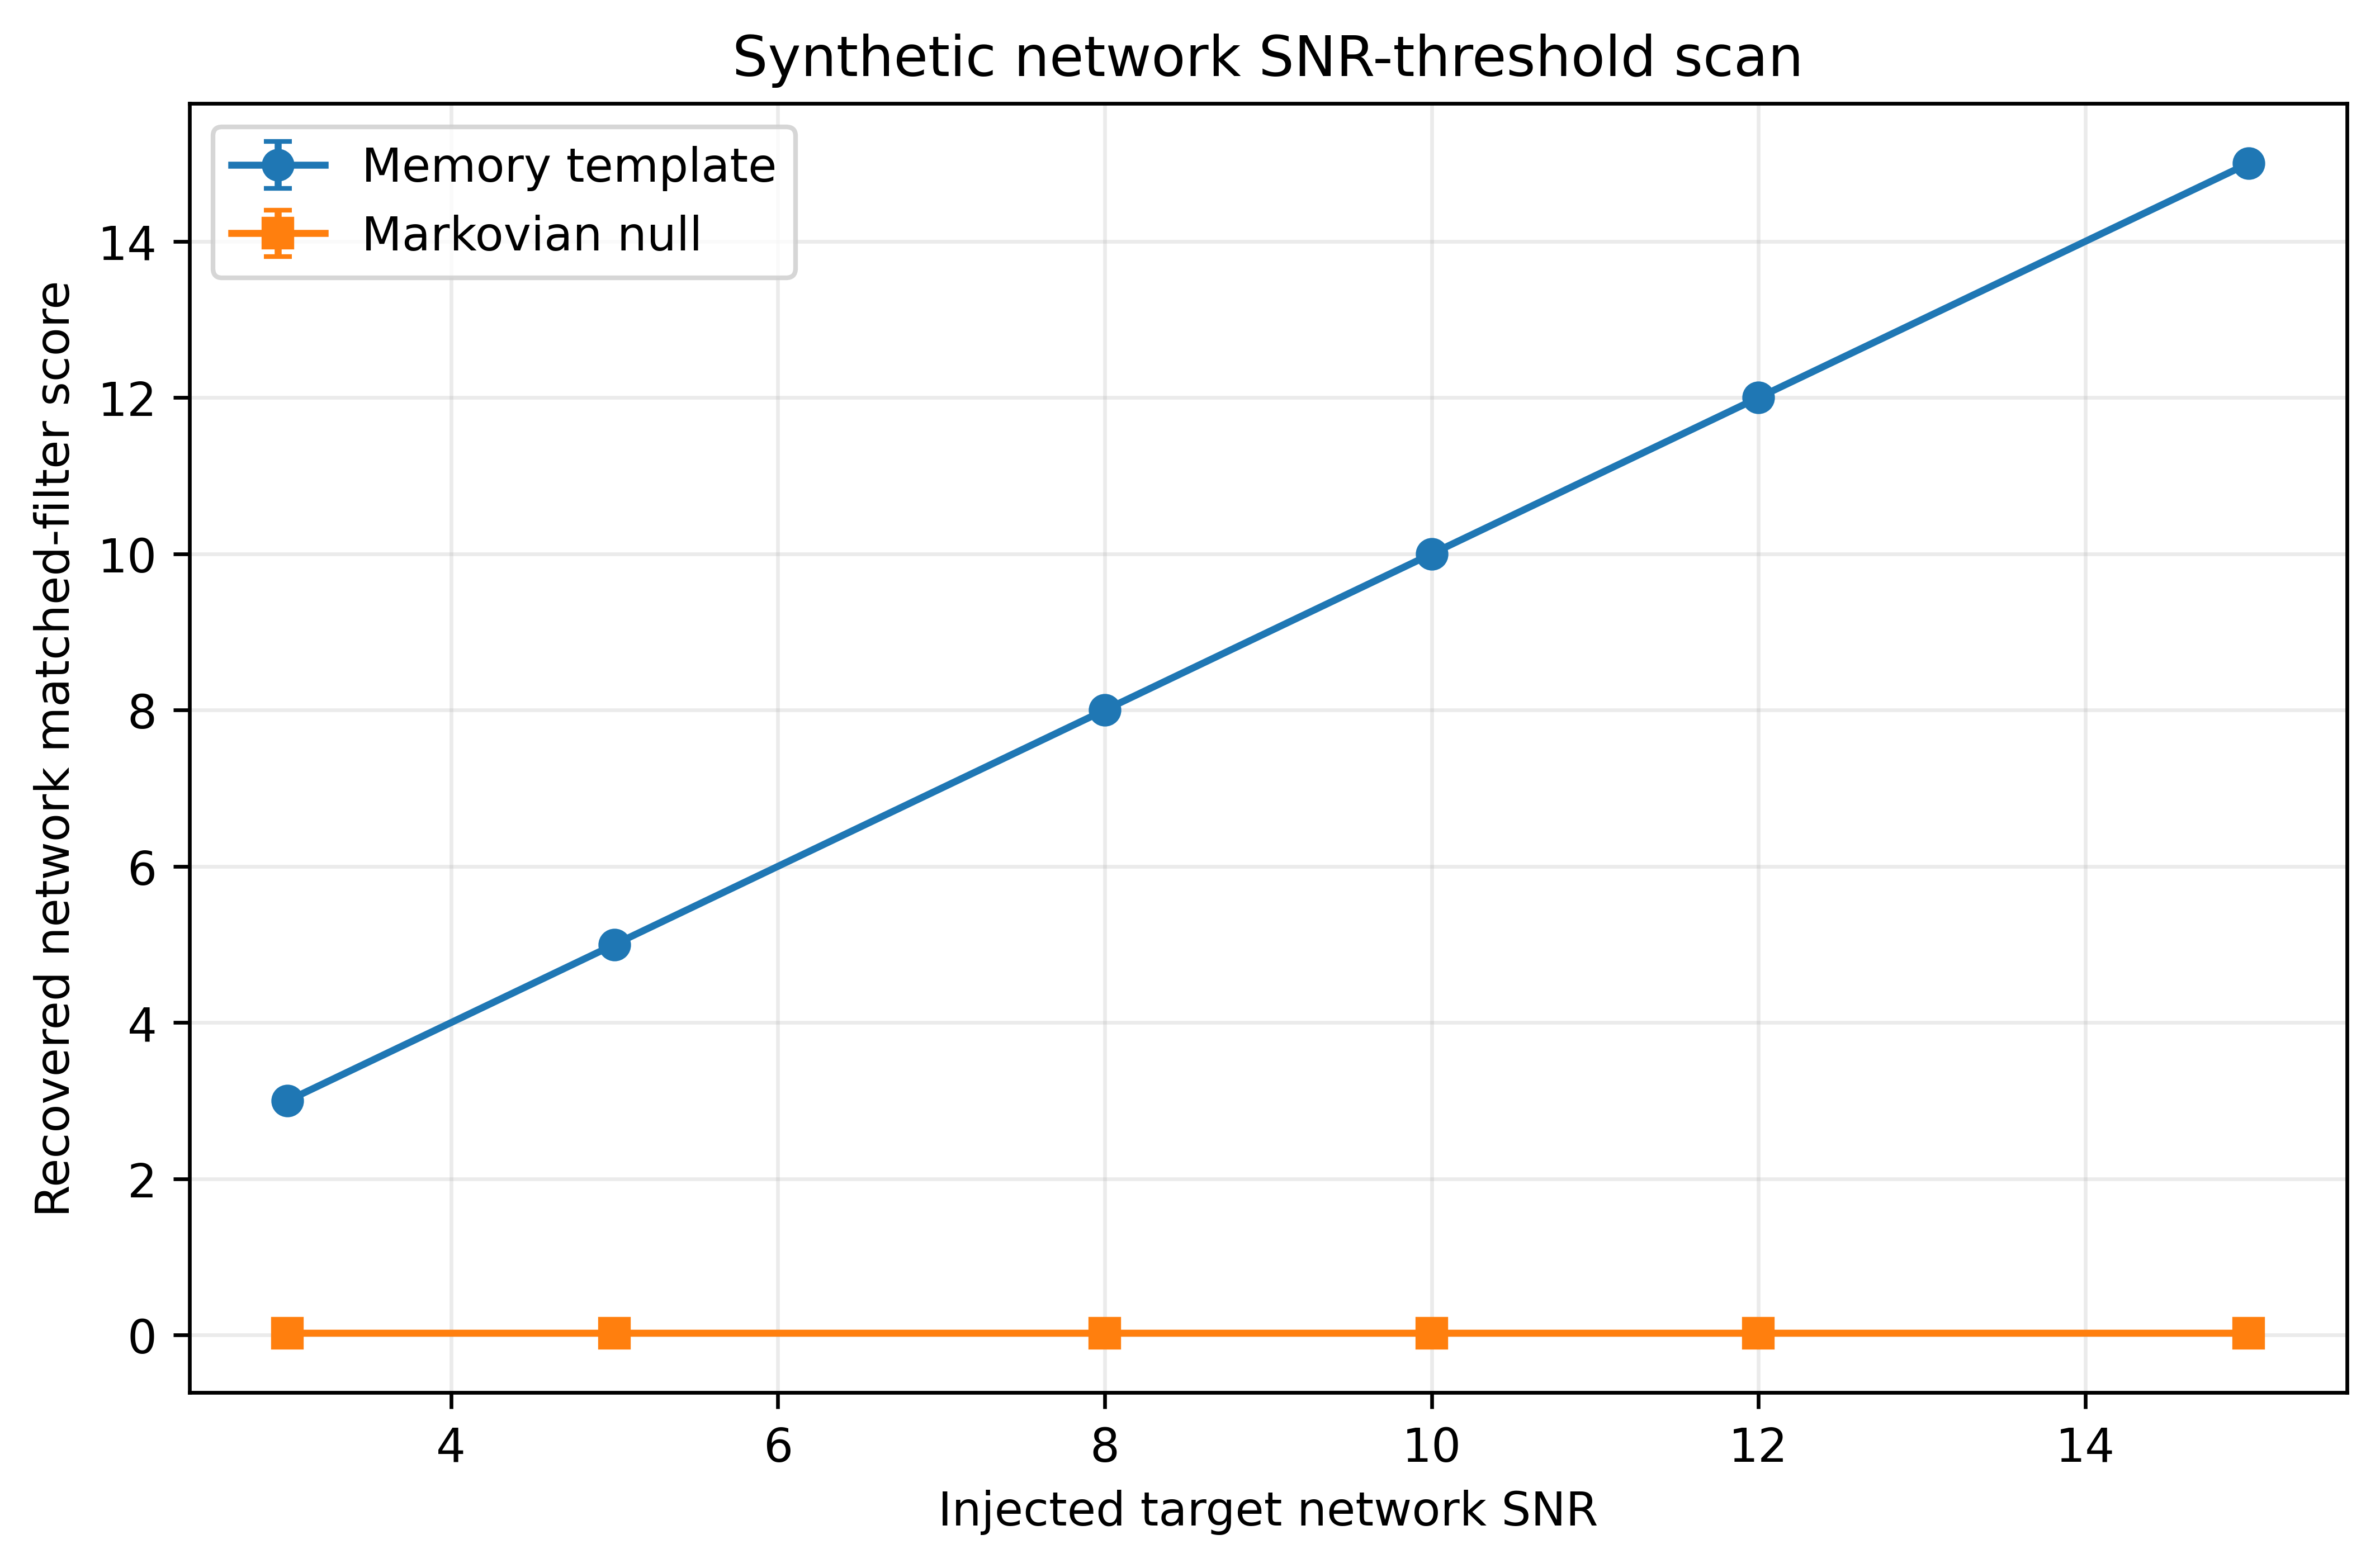
\includegraphics[width=0.86\textwidth]{network_snr_scan/network_snr_threshold_scan.png}
\caption{Synthetic network SNR-threshold scan. The memory-completed template recovers the injected network score across the tested SNR range, while the Markovian-null template remains close to zero.}
\label{fig:network_snr_threshold}
\end{figure}

\begin{figure}[t]
\centering

\includegraphics[width=0.86\textwidth]{network_snr_scan/network_snr_contrast_scan.png}
\caption{Memory-minus-null network contrast as a function of injected network SNR. The contrast scales approximately linearly because the memory waveform proxy is nearly orthogonal to the Markovian-null template under the adopted synthetic-noise model.}
\label{fig:network_snr_contrast}
\end{figure}

\section{Mapping the Anisotropy Proxy to Core-Collapse Quantities}
\label{sec:ccsn_mapping}

The toy anisotropy coordinate \(A(t)\) should be interpreted as a reduced anisotropic-stress proxy, not as a single literal observable. In a core-collapse supernova implementation, a practical mapping is
\begin{equation}
A(t)=w_\nu A_\nu(t)+w_{\rm turb}A_{\rm turb}(t)+w_{\rm rot}A_{\rm rot}(t)+w_{\rm acc}A_{\rm acc}(t),
\end{equation}
where \(A_\nu\) measures angular anisotropy in neutrino luminosity, \(A_{\rm turb}\) measures anisotropic turbulent stress, \(A_{\rm rot}\) measures rotational deformation, and \(A_{\rm acc}\) measures anisotropic accretion.

For example, if \(L_\nu(\theta,\phi,t)\) is the direction-dependent neutrino luminosity, a quadrupolar neutrino-anisotropy proxy can be defined as
\begin{equation}
A_\nu(t)=\frac{1}{L_{\nu,0}(t)}\left[\sum_{m=-2}^{2}\left|\int L_\nu(\theta,\phi,t)Y_{2m}^{\ast}(\theta,\phi)d\Omega\right|^2\right]^{1/2},
\end{equation}
where \(L_{\nu,0}\) is the angular monopole. This construction is useful because gravitational-wave emission is quadrupole-sensitive. It also prevents overinterpretation: \(A(t)\) is a controlled projection from multidimensional radiation-hydrodynamic fields onto the toy coordinate used in the source-memory test.

In a real collapse simulation, \(R(t)\) should likewise be tied to a specified physical radius or compactness measure, such as proto-neutron-star radius, shock radius, or a compactness-growth coordinate. Then \(\dot R^2(t)\) becomes a compression-rate history, while \(A^2(t)\) becomes an anisotropic-stress history. The toy observable \(\Xi(t)=\dot R^2+\beta A^2\) is therefore best understood as a reduced projection of compression and anisotropy history rather than as a primitive astrophysical law.

\section{Toward a \texorpdfstring{\(3+1\)}{3+1} GRHD Implementation}
\label{sec:grhd_implementation}

The scalar toy model is not the final physical representation of collapse. A realistic implementation requires lifting the collapse-state variables into field-valued quantities on a \(3+1\) spacetime foliation. This section gives the corresponding implementation architecture. No full numerical-relativity simulation is claimed.

In the \(3+1\) decomposition,
\begin{equation}
ds^2=-\alpha^2dt^2+\gamma_{ij}\left(dx^i+\beta^i dt\right)\left(dx^j+\beta^j dt\right),
\end{equation}
where \(\alpha\) is the lapse, \(\beta^i\) is the shift, and \(\gamma_{ij}\) is the spatial metric. The scalar state vector is interpreted as a reduced projection of
\begin{equation}
\hat{\Phi}_{\rm coll}(t,\mathbf{x})=\left(\mathcal{H}_{ij},\mathcal{R},\mathcal{S}_{ij},\mathcal{M}_{ij}\right)(t,\mathbf{x}).
\end{equation}
The structural-reserve field \(\mathcal{H}_{ij}\) is associated with local support against runaway collapse, encoded in pressure, anisotropic stress, magnetic stress, or turbulent effective stress. The recoverability field \(\mathcal{R}\) may be constructed from quantities such as the expansion scalar \(\Theta=\nabla_\mu u^\mu\), the determinant \(\gamma=\det(\gamma_{ij})\), lapse collapse, shock-revival diagnostics, or apparent-horizon proximity measures. The coherence field \(\mathcal{S}_{ij}\) may be built from shear, vorticity, turbulent kinetic energy, mode coherence, or shell-crossing diagnostics.

The source-memory variable is introduced as a spatial tensor,
\begin{equation}
\mathcal{M}_{ij}(t,\mathbf{x})=\int_{t_0}^{t}K_M(t,t';\mathbf{x})\,\Xi_{ij}(t',\mathbf{x})\,dt'.
\end{equation}
A minimal history-driving tensor is
\begin{equation}
\Xi_{ij}=\sigma_{ij}+\beta_\omega\omega_{ij}+\beta_\Pi\Pi_{ij},
\end{equation}
where \(\sigma_{ij}\) is a shear-like deformation tensor, \(\omega_{ij}\) is a vorticity-related contribution after spatial projection, and \(\Pi_{ij}\) is anisotropic stress. In a geometric implementation, a natural shear proxy is the trace-free extrinsic curvature,
\begin{equation}
A_{ij}=K_{ij}-\frac{1}{3}\gamma_{ij}K.
\end{equation}
In a fluid implementation, the shear of the fluid congruence may be used,
\begin{equation}
\sigma_{\mu\nu}=h_{\mu}^{\ \alpha}h_{\nu}^{\ \beta}\nabla_{(\alpha}u_{\beta)}-\frac{1}{3}h_{\mu\nu}\Theta,
\qquad
h_{\mu\nu}=g_{\mu\nu}+u_\mu u_\nu.
\end{equation}

For an exponential kernel, the memory tensor can be evolved locally,
\begin{equation}
\partial_t\mathcal{M}_{ij}=\frac{1}{\tau_M}\left(\Xi_{ij}-\mathcal{M}_{ij}\right)+\mathcal{L}_{\beta}\mathcal{M}_{ij}-2\alpha K^k_{\ (i}\mathcal{M}_{j)k}+\mathcal{C}_{ij},
\end{equation}
where \(\mathcal{L}_{\beta}\) is the Lie derivative along the shift and \(\mathcal{C}_{ij}\) represents implementation-dependent constraint cleaning, trace removal, or projection back onto the desired tensor subspace. A conservative first implementation may evolve only the trace-free projection
\begin{equation}
\mathcal{M}^{\rm TF}_{ij}=\mathcal{M}_{ij}-\frac{1}{3}\gamma_{ij}\gamma^{kl}\mathcal{M}_{kl}.
\end{equation}

The memory tensor can enter the matter sector as an effective anisotropic stress. A conservative first implementation restricts the memory contribution to spatial stresses,
\begin{equation}
S_{ij}^{\rm eff}=S_{ij}+\lambda_{\rm mem}\mathcal{M}^{\rm TF}_{ij},
\end{equation}
where \(S_{ij}=\gamma_i^{\ \mu}\gamma_j^{\ \nu}T_{\mu\nu}\). In conservative GRHD form,
\begin{equation}
\partial_t\mathbf{U}+\partial_i\mathbf{F}^i=\mathbf{S}_{\rm GRHD}+\lambda_{\rm mem}\mathbf{S}_{\rm mem},
\end{equation}
with a schematic source structure
\begin{equation}
\mathbf{S}_{\rm mem}=\begin{bmatrix}
0 \\
-\alpha\sqrt{\gamma}\nabla_j\mathcal{M}^{j}{}_{i} \\
-\alpha\sqrt{\gamma}\mathcal{M}^{ij}K_{ij}
\end{bmatrix}.
\end{equation}
The zero in the rest-mass row enforces baryon conservation. The momentum term represents divergence of effective anisotropic memory stress. The energy term represents work done by memory stress against slice deformation. This is an implementation-level ansatz requiring tests of hyperbolicity, stability, constraint preservation, and convergence.

Waveform extraction should remain standard. The memory tensor is not a replacement for \(\Psi_4\). It is a source-side field that changes the evolution of matter and geometry, thereby changing the extracted waveform. The observable test is
\begin{equation}
\Delta\Psi_4=\Psi_4[\lambda_{\rm mem}\neq0]-\Psi_4[\lambda_{\rm mem}=0],
\end{equation}
or equivalently \(\Delta h=h[\lambda_{\rm mem}\neq0]-h[\lambda_{\rm mem}=0]\), under matched initial or intermediate-state conditions.

\begin{table}[t]
\centering
\caption{Conceptual uplift from the scalar toy model to a field-valued \(3+1\) GRHD implementation.}
\begin{tabular}{lll}
\toprule
Toy variable & Physical role & \(3+1\) implementation candidate \\
\midrule
\(H_{\rm coll}\) & Structural reserve & spatial stress \(S_{ij}\), pressure, magnetic stress, anisotropic stress \\
\(R_{\rm coll}\) & Recoverability & \(\Theta\), lapse collapse, \(\det\gamma_{ij}\), shock-revival or horizon-proximity diagnostics \\
\(S_{\rm coll}\) & Coherence & shear, vorticity, turbulent kinetic energy, mode coherence \\
\(M_{\rm coll}\) & Retained history & memory tensor \(\mathcal{M}_{ij}\) driven by \(A_{ij}\), \(\sigma_{ij}\), \(\omega_{ij}\), or \(\Pi_{ij}\) \\
\bottomrule
\end{tabular}
\label{tab:grhd_uplift}
\end{table}

A numerical implementation should proceed in stages. First, evolve \(\mathcal{M}_{ij}\) passively with \(\lambda_{\rm mem}=0\) to verify boundedness and convergence on fixed collapse backgrounds. Second, activate weak back-reaction through effective stress sources and test controlled relativistic shocks, spherical collapse, and rotating-core benchmarks. Third, compare matched-state collapse histories with different prior shear histories and extract \(\Psi_4\) at large radius. The framework is supported only if waveform residuals persist after conditioning on the extended instantaneous state and correlate with \(\mathcal{M}_{ij}\).

\section{Reproducibility}
\label{sec:reproducibility}

The executable validation was organized as a reproducible source tree. To make the numerical tables traceable to the text, the code token \texttt{delta\_match\_after\_reset} corresponds to the matched-state diagnostic \(\delta_{\rm match}\), \texttt{delta\_M\_at\_tstar} corresponds to \(\Delta M_{\rm coll}(t_\ast)\), \texttt{post\_delta\_h\_norm} corresponds to the waveform-residual norm \(\mathcal{R}_h\), and \texttt{mean\_delta\_network\_rho} corresponds to the memory-minus-null network contrast. The relevant scripts are \texttt{scripts/01\_run\_toy\_model.py}, \texttt{scripts/03\_run\_fixed\_history\_lambda\_scan.py}, \texttt{scripts/04\_compare\_baseline\_amplified.py}, \texttt{scripts/05\_make\_manuscript\_grade\_plots.py}, \texttt{scripts/06\_synthetic\_detector\_injection.py}, \texttt{scripts/07\_summarize\_detector\_degeneracy.py}, \texttt{scripts/08\_multidetector\_coincident\_analysis.py}, \texttt{scripts/09\_compare\_network\_glitch.py}, \texttt{scripts/10\_run\_network\_snr\_scan.py}, and \texttt{scripts/11\_plot\_network\_snr\_scan.py}. The main configurations are \texttt{configs/toy\_model\_baseline.yaml}, \texttt{configs/toy\_model\_amplified\_history.yaml}, \texttt{configs/synthetic\_detector\_injection.yaml}, \texttt{configs/multidetector\_network.yaml}, and \texttt{configs/multidetector\_network\_noglitch.yaml}. The key output tables are \texttt{results/toy\_model\_comparison.csv}, \texttt{results/synthetic\_detector/synthetic\_detector\_summary.csv}, \texttt{results/synthetic\_detector/synthetic\_detector\_degeneracy\_summary.csv}, \texttt{results/network\_glitch\_comparison.csv}, and \texttt{results/network\_snr\_threshold\_scan.csv}.

The toy and detector calculations use dimensionless waveform proxies and synthetic colored-noise models. Therefore, the numerical values should be interpreted as internal validation diagnostics, not as astrophysical rate, distance, or detector-sensitivity forecasts. The reproducibility claim is limited to regenerating the toy trajectories, residuals, synthetic injections, network summaries, and manuscript figures from the stated scripts and configurations.

\section{Limitations}
\label{sec:limitations}

Several limitations are explicit. First, the toy model is scalar and dimensionless. It demonstrates path dependence under controlled matching, but it is not a relativistic hydrodynamic simulation. Second, the waveform proxy is quadrupole-inspired and diagnostic. It is not a substitute for \(\Psi_4\), Cauchy-characteristic extraction, or calibrated waveform extraction. Third, the synthetic detector tests use analytic colored noise and controlled antenna factors. They demonstrate separability from the Markovian null in the constructed toy waveform space, not real detector detectability. Fourth, nonzero memory templates are highly degenerate with each other in the present waveform family. The detector analysis supports memory-on versus memory-off separation, not precision inference of \(\lambda_{\rm mem}\). This is best interpreted as a flat direction in the scalar template space rather than as failure of the memory-on test. It also motivates the field-valued extension: a scalar amplitude-like coupling is unlikely to carry enough structure to resolve detailed source-history parameters. Fifth, the \(3+1\) GRHD section is an implementation architecture. It defines how the memory tensor could be inserted into future solvers, but it does not report such a solver.

These limitations are not incidental. They define the falsifiability boundary. The theory is weakened if residuals disappear after conditioning on an enlarged instantaneous state, if source memory cannot be stably evolved in field form, if memory back-reaction violates numerical stability or conservation constraints, or if realistic waveform extraction shows no source-history-correlated residuals.

\section{Discussion}
\label{sec:discussion}

The central result is methodological. The source-memory hypothesis has been reduced to a controlled test: same instantaneous state, different retained history, different subsequent waveform residual only when memory is dynamically active. The amplified toy run supplies a strong example of this structure, while the detector and network analyses show that the resulting residual is not merely a visual artifact of the toy trajectory. Under the adopted synthetic noise model, the residual is nearly orthogonal to the Markovian null.

The strongest interpretation is also the narrowest. The paper does not show that astrophysical gravitational collapse is non-Markovian. It shows that an effective non-Markovian source description is mathematically coherent, executable, falsifiable, and extendable to a \(3+1\) implementation architecture. The model survives the first internal checks that a theory of source-side memory should survive: matched-state control, fixed-history coupling scan, null-template rejection, network projection, SNR-threshold scaling, glitch-leakage accounting, and explicit degeneracy accounting.

The framework also clarifies how source-side memory and gravitational-wave memory should be kept separate. Source-side memory is a retained internal history coordinate of the source. Gravitational-wave memory is a radiative spacetime effect. The former may alter the latter, but the concepts are not identical. Keeping this distinction prevents the theory from relying on terminology rather than mechanism.

A future numerical relativity implementation would be the decisive next step. The minimal useful test would not be a generic collapse simulation. It would be a matched-state experiment in which two collapse histories are brought to the same extended instantaneous state while retaining different \(\mathcal{M}_{ij}\) fields, followed by waveform extraction through \(\Psi_4\). If residuals remain and correlate with the memory tensor, source-side non-Markovian collapse would become a concrete numerical-relativity hypothesis. If residuals vanish, the framework would identify the conditions under which collapse is effectively Markovian.

\section{Conclusion}

This paper has proposed a non-Markovian state-space framework for gravitational collapse. A causal source-memory coordinate was introduced and embedded within a collapse-state vector consisting of reserve, recoverability, coherence, and memory. The scalar model was tested through exact matched-state resetting, fixed-history memory-coupling scans, synthetic colored-noise injection, and a three-detector network architecture. The strongest toy result shows that a fixed retained memory contrast produces negligible waveform residuals when memory is inactive and a monotonic residual when memory is coupled to collapse evolution. The detector and network tests show strong separation between the memory-completed residual and the Markovian null under the adopted synthetic assumptions.

The paper also specifies how the scalar framework can be lifted into a field-valued \(3+1\) GRHD architecture through a memory tensor \(\mathcal{M}_{ij}\), effective anisotropic stress coupling, and standard waveform extraction. This second phase is not claimed as a completed numerical-relativity implementation. It is an implementation map. The immediate implication is disciplined: gravitational collapse should be tested not only by asking what the source is at a given instant, but also by asking whether its prior path remains dynamically observable.


\begin{thebibliography}{99}

\bibitem{Abbott2016GW150914}
B. P. Abbott et al. (LIGO Scientific Collaboration and Virgo Collaboration), ``Observation of gravitational waves from a binary black hole merger,'' \emph{Physical Review Letters} \textbf{116}, 061102 (2016). doi:10.1103/PhysRevLett.116.061102.

\bibitem{Belgacem2018ModifiedGW}
E. Belgacem, Y. Dirian, S. Foffa, and M. Maggiore, ``Modified gravitational-wave propagation and standard sirens,'' \emph{Physical Review D} \textbf{98}, 023510 (2018). doi:10.1103/PhysRevD.98.023510.

\bibitem{Belgacem2019TestingMG}
E. Belgacem et al., ``Testing modified gravity at cosmological distances with LISA standard sirens,'' \emph{Journal of Cosmology and Astroparticle Physics} \textbf{2019}, 024 (2019). doi:10.1088/1475-7516/2019/07/024.

\bibitem{Tagliazucchi2025StandardSiren}
M. Tagliazucchi et al., ``Accelerating the standard siren method: improved constraints on modified gravitational-wave propagation with future data,'' \emph{Astronomy \& Astrophysics} (2025). doi:10.1051/0004-6361/202554827.

\bibitem{Muller2017CCSN}
B. M{\"u}ller, ``Gravitational waves from core-collapse supernovae,'' \emph{Proceedings of the International Astronomical Union} \textbf{12}, 165--174 (2017). doi:10.1017/S1743921317004285.

\bibitem{Muller2026CCSNReview}
B. M{\"u}ller, ``Core-collapse supernovae and their gravitational wave signals: the status of theory and modeling,'' arXiv:2603.24243 (2026).

\bibitem{Murphy2026Progenitor}
R. Daniel Murphy, E. Brinkman, C. J. Richardson, E. Semenak, A. Mezzacappa, P. Marronetti, E. J. Lentz, and S. W. Bruenn, ``Gravitational waves as a probe of core collapse supernova progenitor structure,'' \emph{Physical Review D} \textbf{113}, 084004 (2026). doi:10.1103/2bdz-783t.

\bibitem{Favata2010Memory}
M. Favata, ``The gravitational-wave memory effect,'' \emph{Classical and Quantum Gravity} \textbf{27}, 084036 (2010). doi:10.1088/0264-9381/27/8/084036.

\bibitem{Lasky2016Memory}
P. D. Lasky, E. Thrane, Y. Levin, J. Blackman, and Y. Chen, ``Detecting gravitational-wave memory with LIGO: implications of GW150914,'' \emph{Physical Review Letters} \textbf{117}, 061102 (2016). doi:10.1103/PhysRevLett.117.061102.

\bibitem{Cogez2026LISAMemory}
A. Cogez et al., ``Detectability of gravitational-wave memory with LISA: a Bayesian approach,'' arXiv:2601.23230 (2026).

\bibitem{Gasparotto2026BeyondGRMemory}
S. Gasparotto et al., ``Gravitational-wave memory in beyond GR theories,'' arXiv:2605.07879 (2026).

\end{thebibliography}

\end{document}
